
\subsection{Algorithm Performance}
The introduced algorithm is a greedy approach and might lead to sub-optimal solutions for the defined problem. Test systems were set up to test the algorithm's time and result performance for selecting four restraints. The comparison was made to two different brute force approaches, providing an optimal solution regarding the optimized metric. One brute force approach maximized the distance of all selected COG of restraints to each other, and the other brute force approach used the CHV spanned by the selected restraints. The test systems were toy models consisting of two strongly overlapping particle clouds. The toy models varied in the number of randomly placed particles.  Each particle could be understood as an atom of a hypothetical molecule that might be selected to be restrained. No further atom-filtering was applied to the toy models, such that all particles of one cloud could be potentially linked to any atom in the other cloud.

The greedy approach's benefit becomes clear regarding time complexity because the exponential scaling of the brute force approaches takes very long and makes the practical use for larger molecules nearly impossible. For selecting four restraints from a 20 particles toy model, the brute force approach requires 1min 56s, and for a 30 particle system, 78 min 29s are already required. However, the greedy approach requires for the 28 particles only 0.031s.

The distance metric's comparison shows that the brute force approach optimizing for the maximal distance between all COG of the selected restraints yields the best results with the largest distances. The second brute force approach, optimizing for the CHV, and our greedy approach show very close results to the optimal approach. On the other side, with a 100 times random pick, the negative control is significantly far from the other approaches. We conclude that all three approaches are very good in maximizing the distance between the selected restraints.

Second, we compared the approaches based on the CHV generated by the selected restraints. Again, the brute force optimizing for this criterion is showing the best results. The two other approaches are again close to each other. Nevertheless, as the number of particles increases, a growing difference in the CHVs of the two approaches to the optimal solution can be observed. On the one hand, this difference growing effect might derive from the growing number of possible choices, on the other, from the suboptimal algorithmic metric used in both approaches based on distances. However, all approaches are well distinguishable from the random approach.

The introduced greedy algorithm can be seen as a trade-off between optimizing a metric and time. It is the fastest algorithm and yields good results in the constraints of the used metrics. We expect the practical usage for restraining two small molecules with the algorithm will usually have eight to ten particles. This amount of particles requires approximately $1$~min for the brute force approaches to restrain two molecules to each other and less than $0.02$~s for the greedy approach. 
%%Convex Hull optimization
\begin{figure}[H]
    \centering
    \begin{subfigure}{0.45\columnwidth}
        \includegraphics[width=\textwidth]{fig/results/algorithm/algorithms_timings.png}
        \caption{}
        \label{fig: time_algorithms}
    \end{subfigure}
    \begin{subfigure}{0.45\columnwidth}
        \includegraphics[width=\textwidth]{fig/results/algorithm/restraint_volumes_algorithms.png}
        \caption{}
        \label{fig: ch_algorithms}
    \end{subfigure}
    \begin{subfigure}{0.45\columnwidth}
        \includegraphics[width=\textwidth]{fig/results/algorithm/restraint_distance_algorithms.png}
        \caption{}
        \label{fig: dist_algorithms}
    \end{subfigure}\\
    \begin{subfigure}{0.45\columnwidth}
        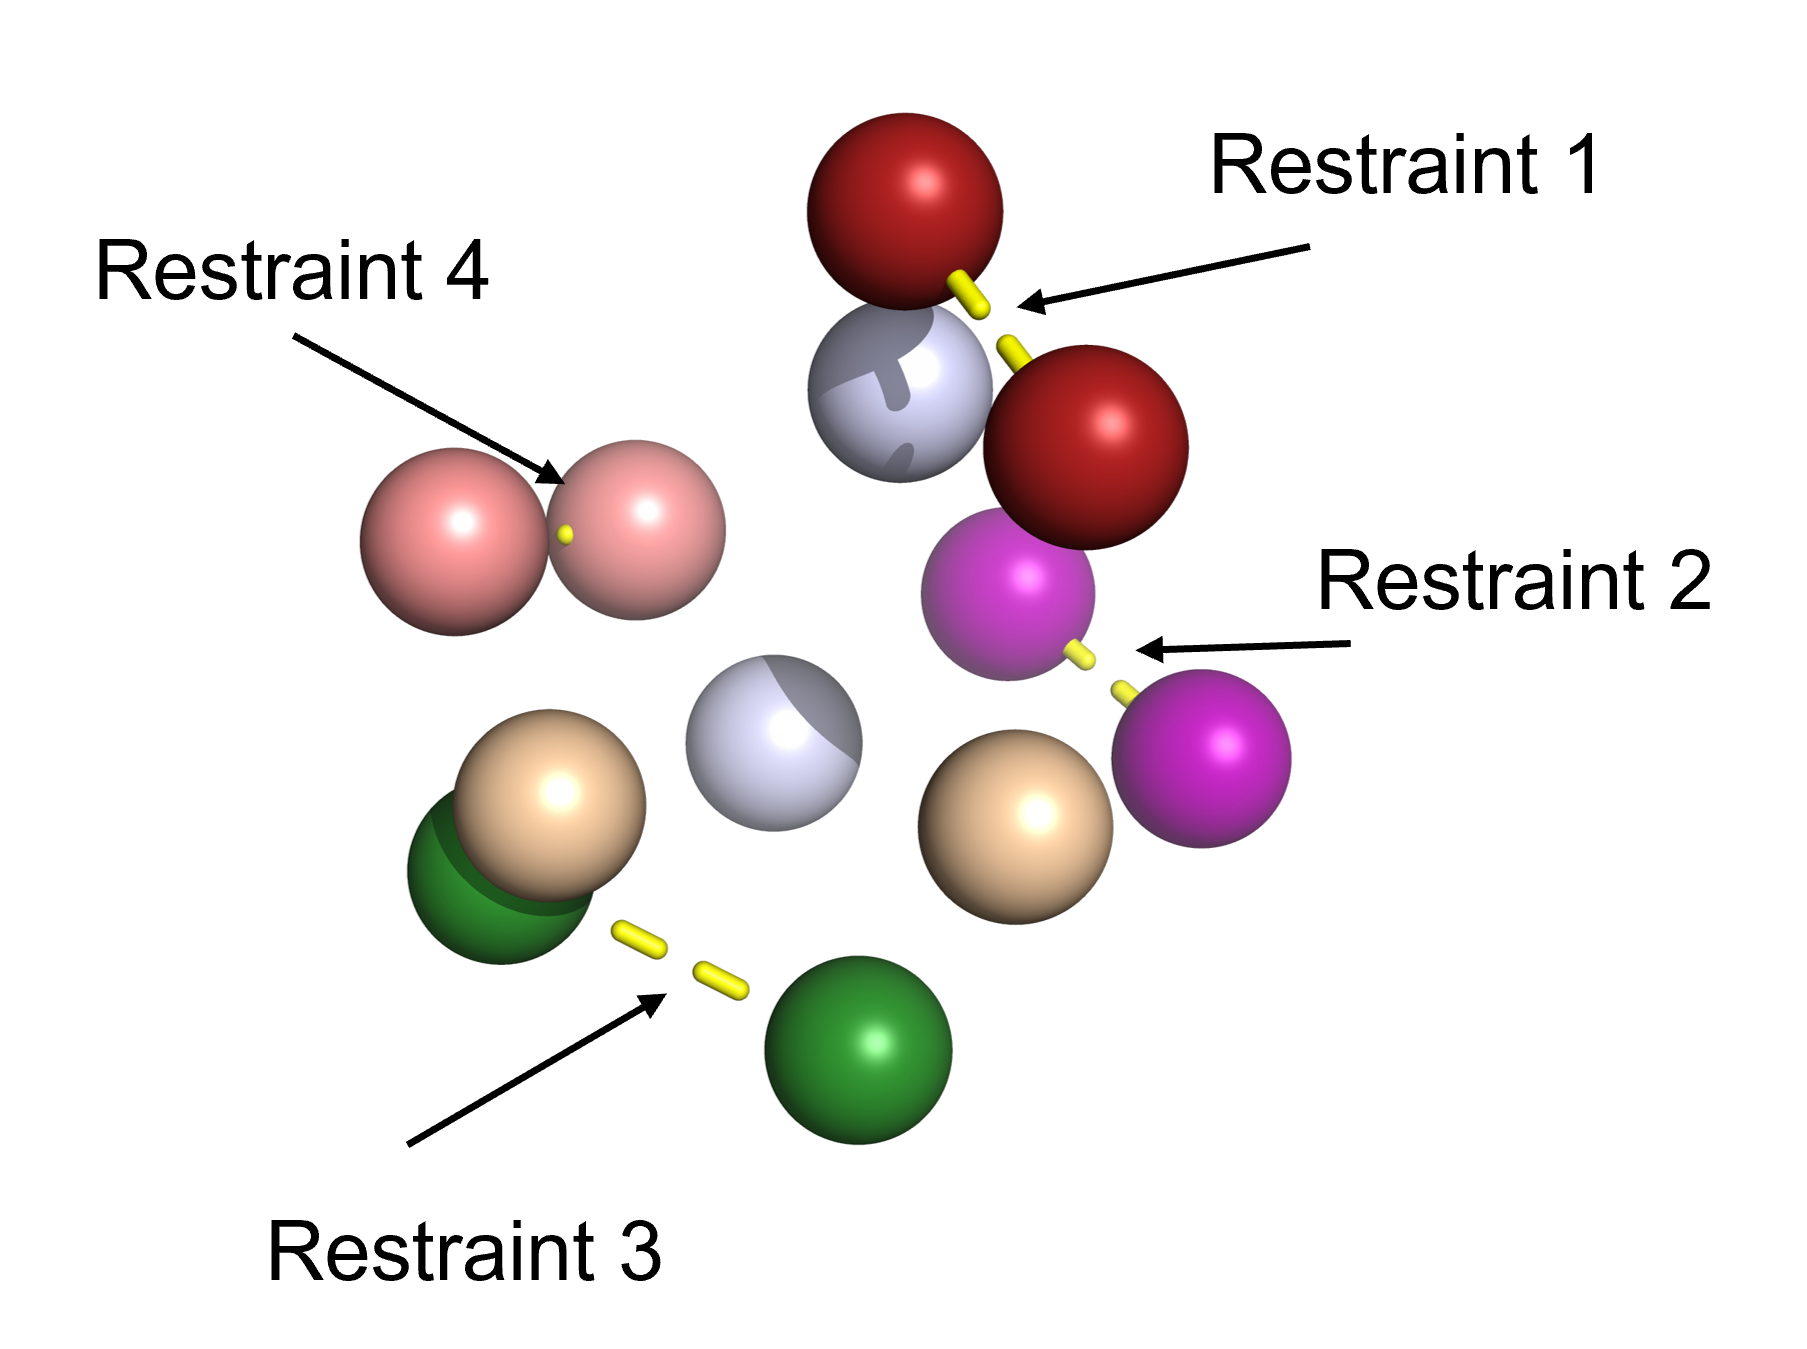
\includegraphics[width=\textwidth]{fig/results/algorithm/punktewolke_6_greedy_annotated.png}
        \caption{}
        \label{fig: greedyApproach_6Partikels}
    \end{subfigure}
    \begin{subfigure}{0.45\columnwidth}
        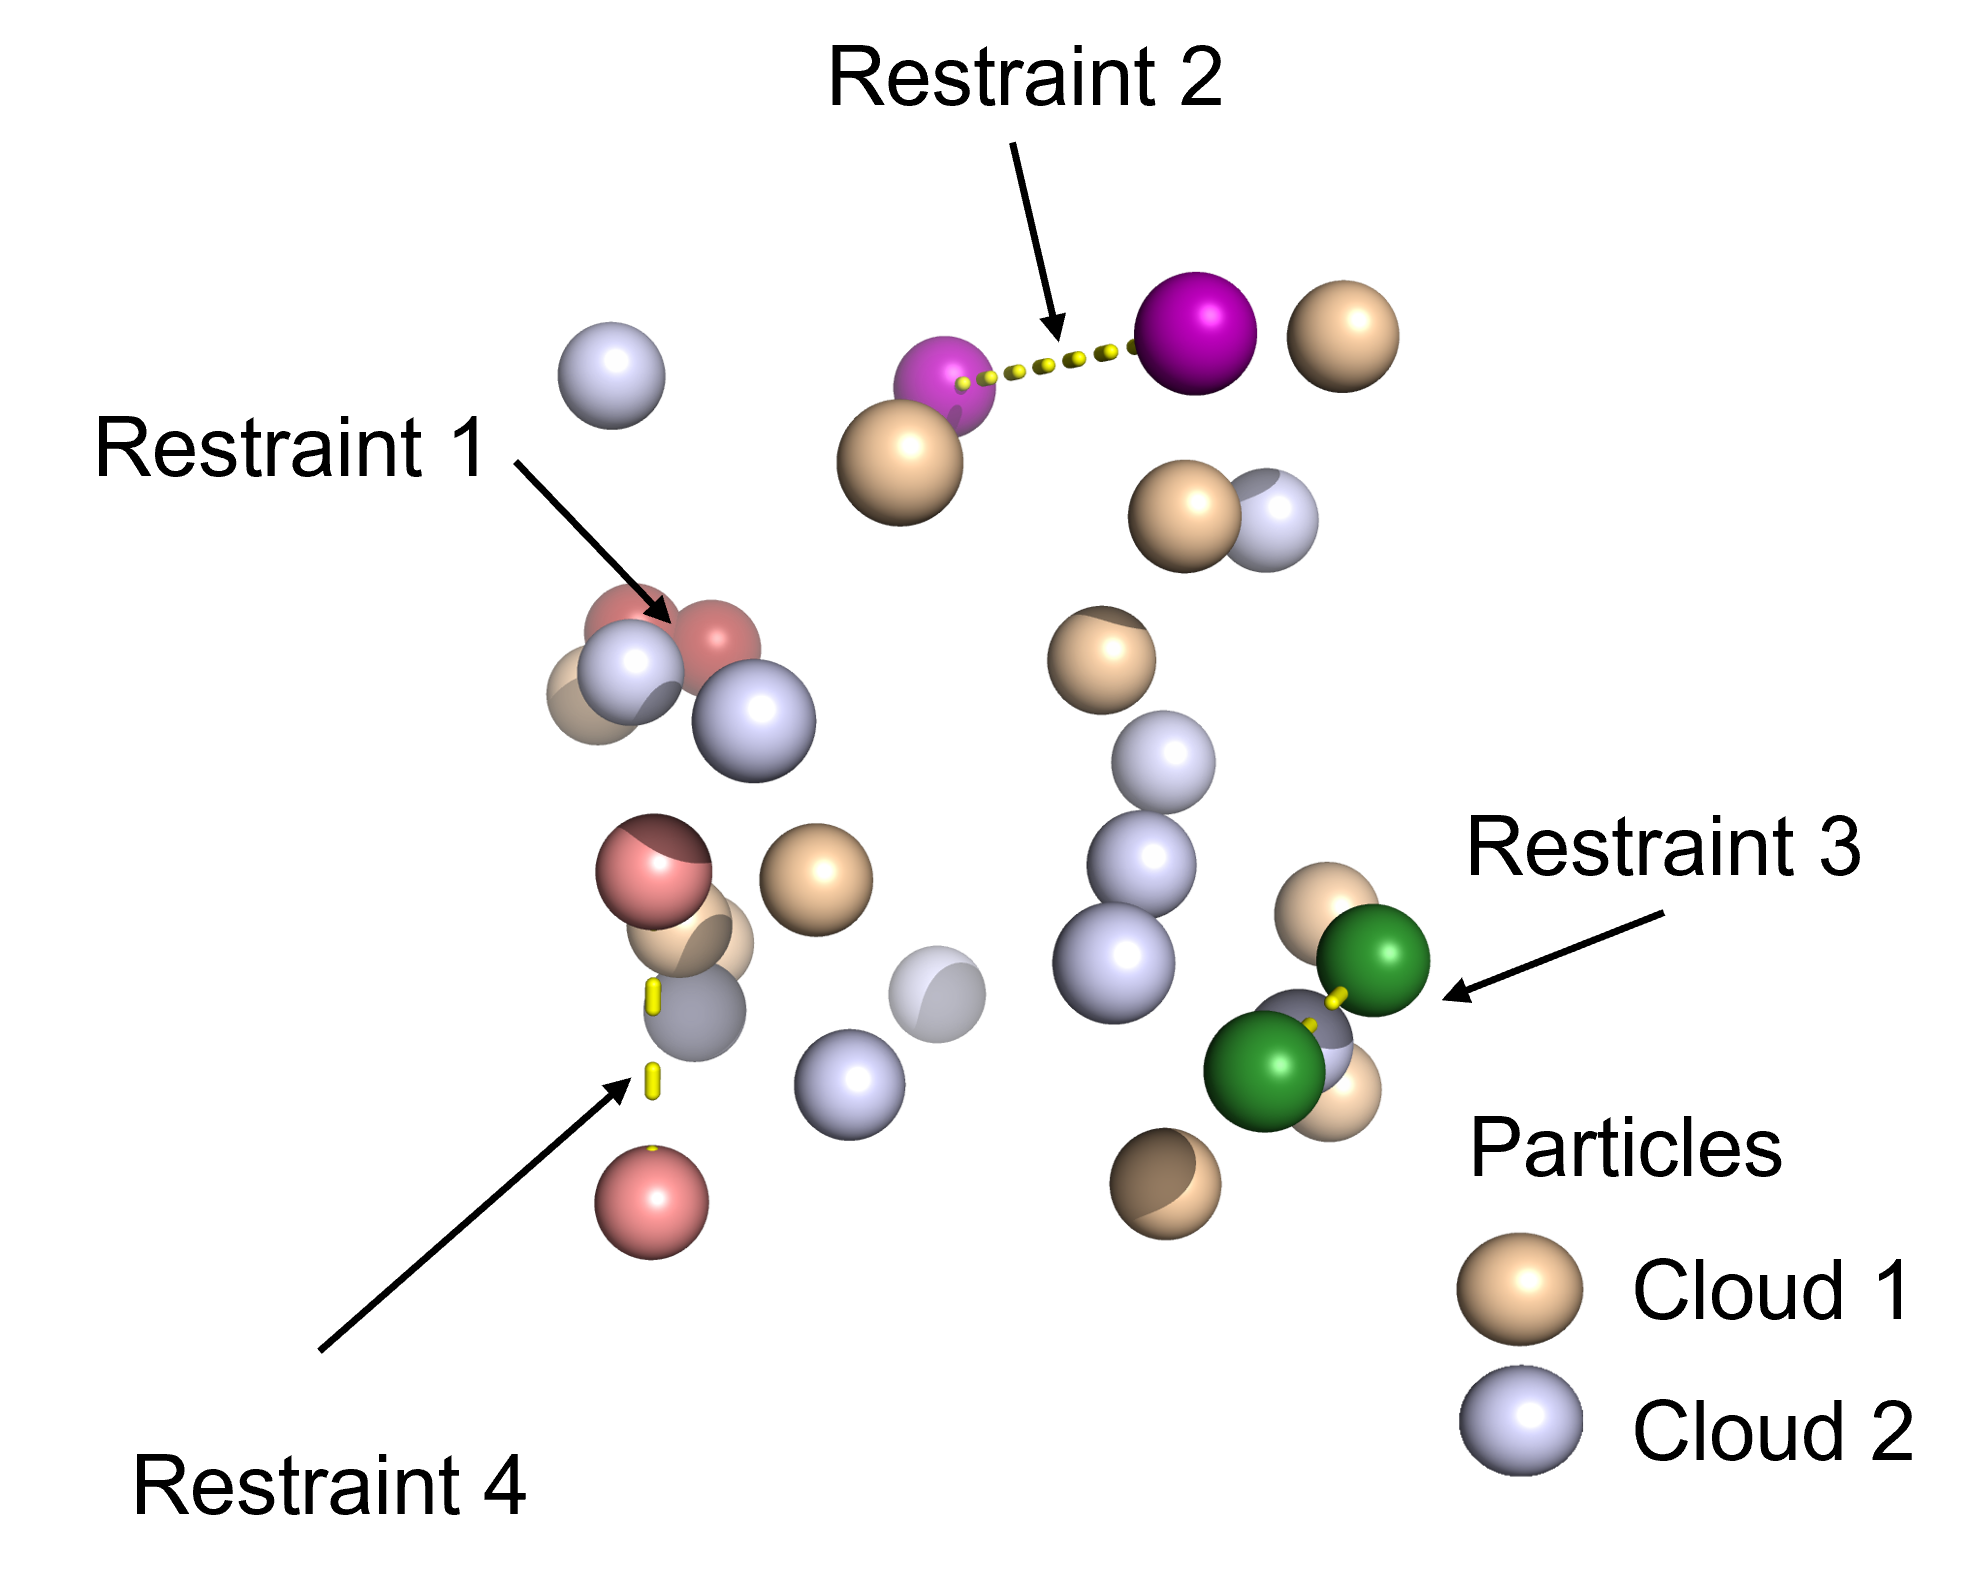
\includegraphics[width=\textwidth]{fig/results/algorithm/punktewolke_15_greedy_annotated.png}
        \caption{}
        \label{fig: greedyApproach_15Partikels}
    \end{subfigure}
    \caption{\ref{fig: time_algorithms} The time complexity of the brute force approaches versus the time complexity of the suggested greedy approach is shown. The selection results can be compared with the generated CHV of the chosen restraints \ref{fig: ch_algorithms} giving insights into the quality of selected atoms.  \ref{fig: greedyApproach_15Partikels} and \ref{fig: greedyApproach_6Partikels} The selection results of the greedy algorithm are visualized to give an impression on the algorithm results. The chosen restraints are colored in green, red, pink and rose and pairwise connected by yellow dashed lines. The two particle clouds are colored in wheat and light blue. }
    \label{fig: ToyMOdelResults}
\end{figure}


\subsection{Pairwise relative hydration free energy calculations}
In order to assess the quality of the distance restraints, the defined algorithm was tested with three test systems derived from the ATB-Server for hydration free energy calculations. \cite{Martin2018} The first FE-Graph (Fig. \ref{fig: Pairwise_TI_M030_Graph}) was calculated in a pairwise star-map layout with the molecule \textit{M030} as the core structure. 

%Free Energy Calculation
\paragraph{Free Energy Calculation}
The resulting relative hydration free energies from the TI-approaches fit very well with the experimental results \cite{Martin2018} with an RMSE of $4.2$~kJ/mol and a MAE of $3.1$~kJ/mol. Subsequently is the ranking of the hydration free energies reasonably well with an $r^2_{spearman} = 0.87$. However, this correlation needs to be taken with a grain of salt, as not the complete hydration free energy graph was calculated and therefore the ranking of the molecules might be influenced by the selection of calculated edges (Figure \ref{fig: pairCorr}). 
In comparison, the results from the ATB server derived via absolute free energy (ABFE) calculations deviate more from the experimental results with an RMSE of $6.7$~kJ/mol and a MAE of $5.5$~kJ/mol, but show a similar ranking correlation of $r^2_{spearman} = 0.84$.
Additionally, due to the adaptive simulation scheme of the ATB server, it is very difficult to compare the spent computational time. Nevertheless, it is very interesting to observe that the molecule pair 6J29 - M030 show in both the ATB approach and the TI approach a similar deviation of $10.7$~kJ\/mol and $12.1$~kJ\/mol, toward the experiment, which hints at a possible force field problem. (Table \ref{SITab: FE_M030_Graph})

\begin{figure}[h]
    \centering
    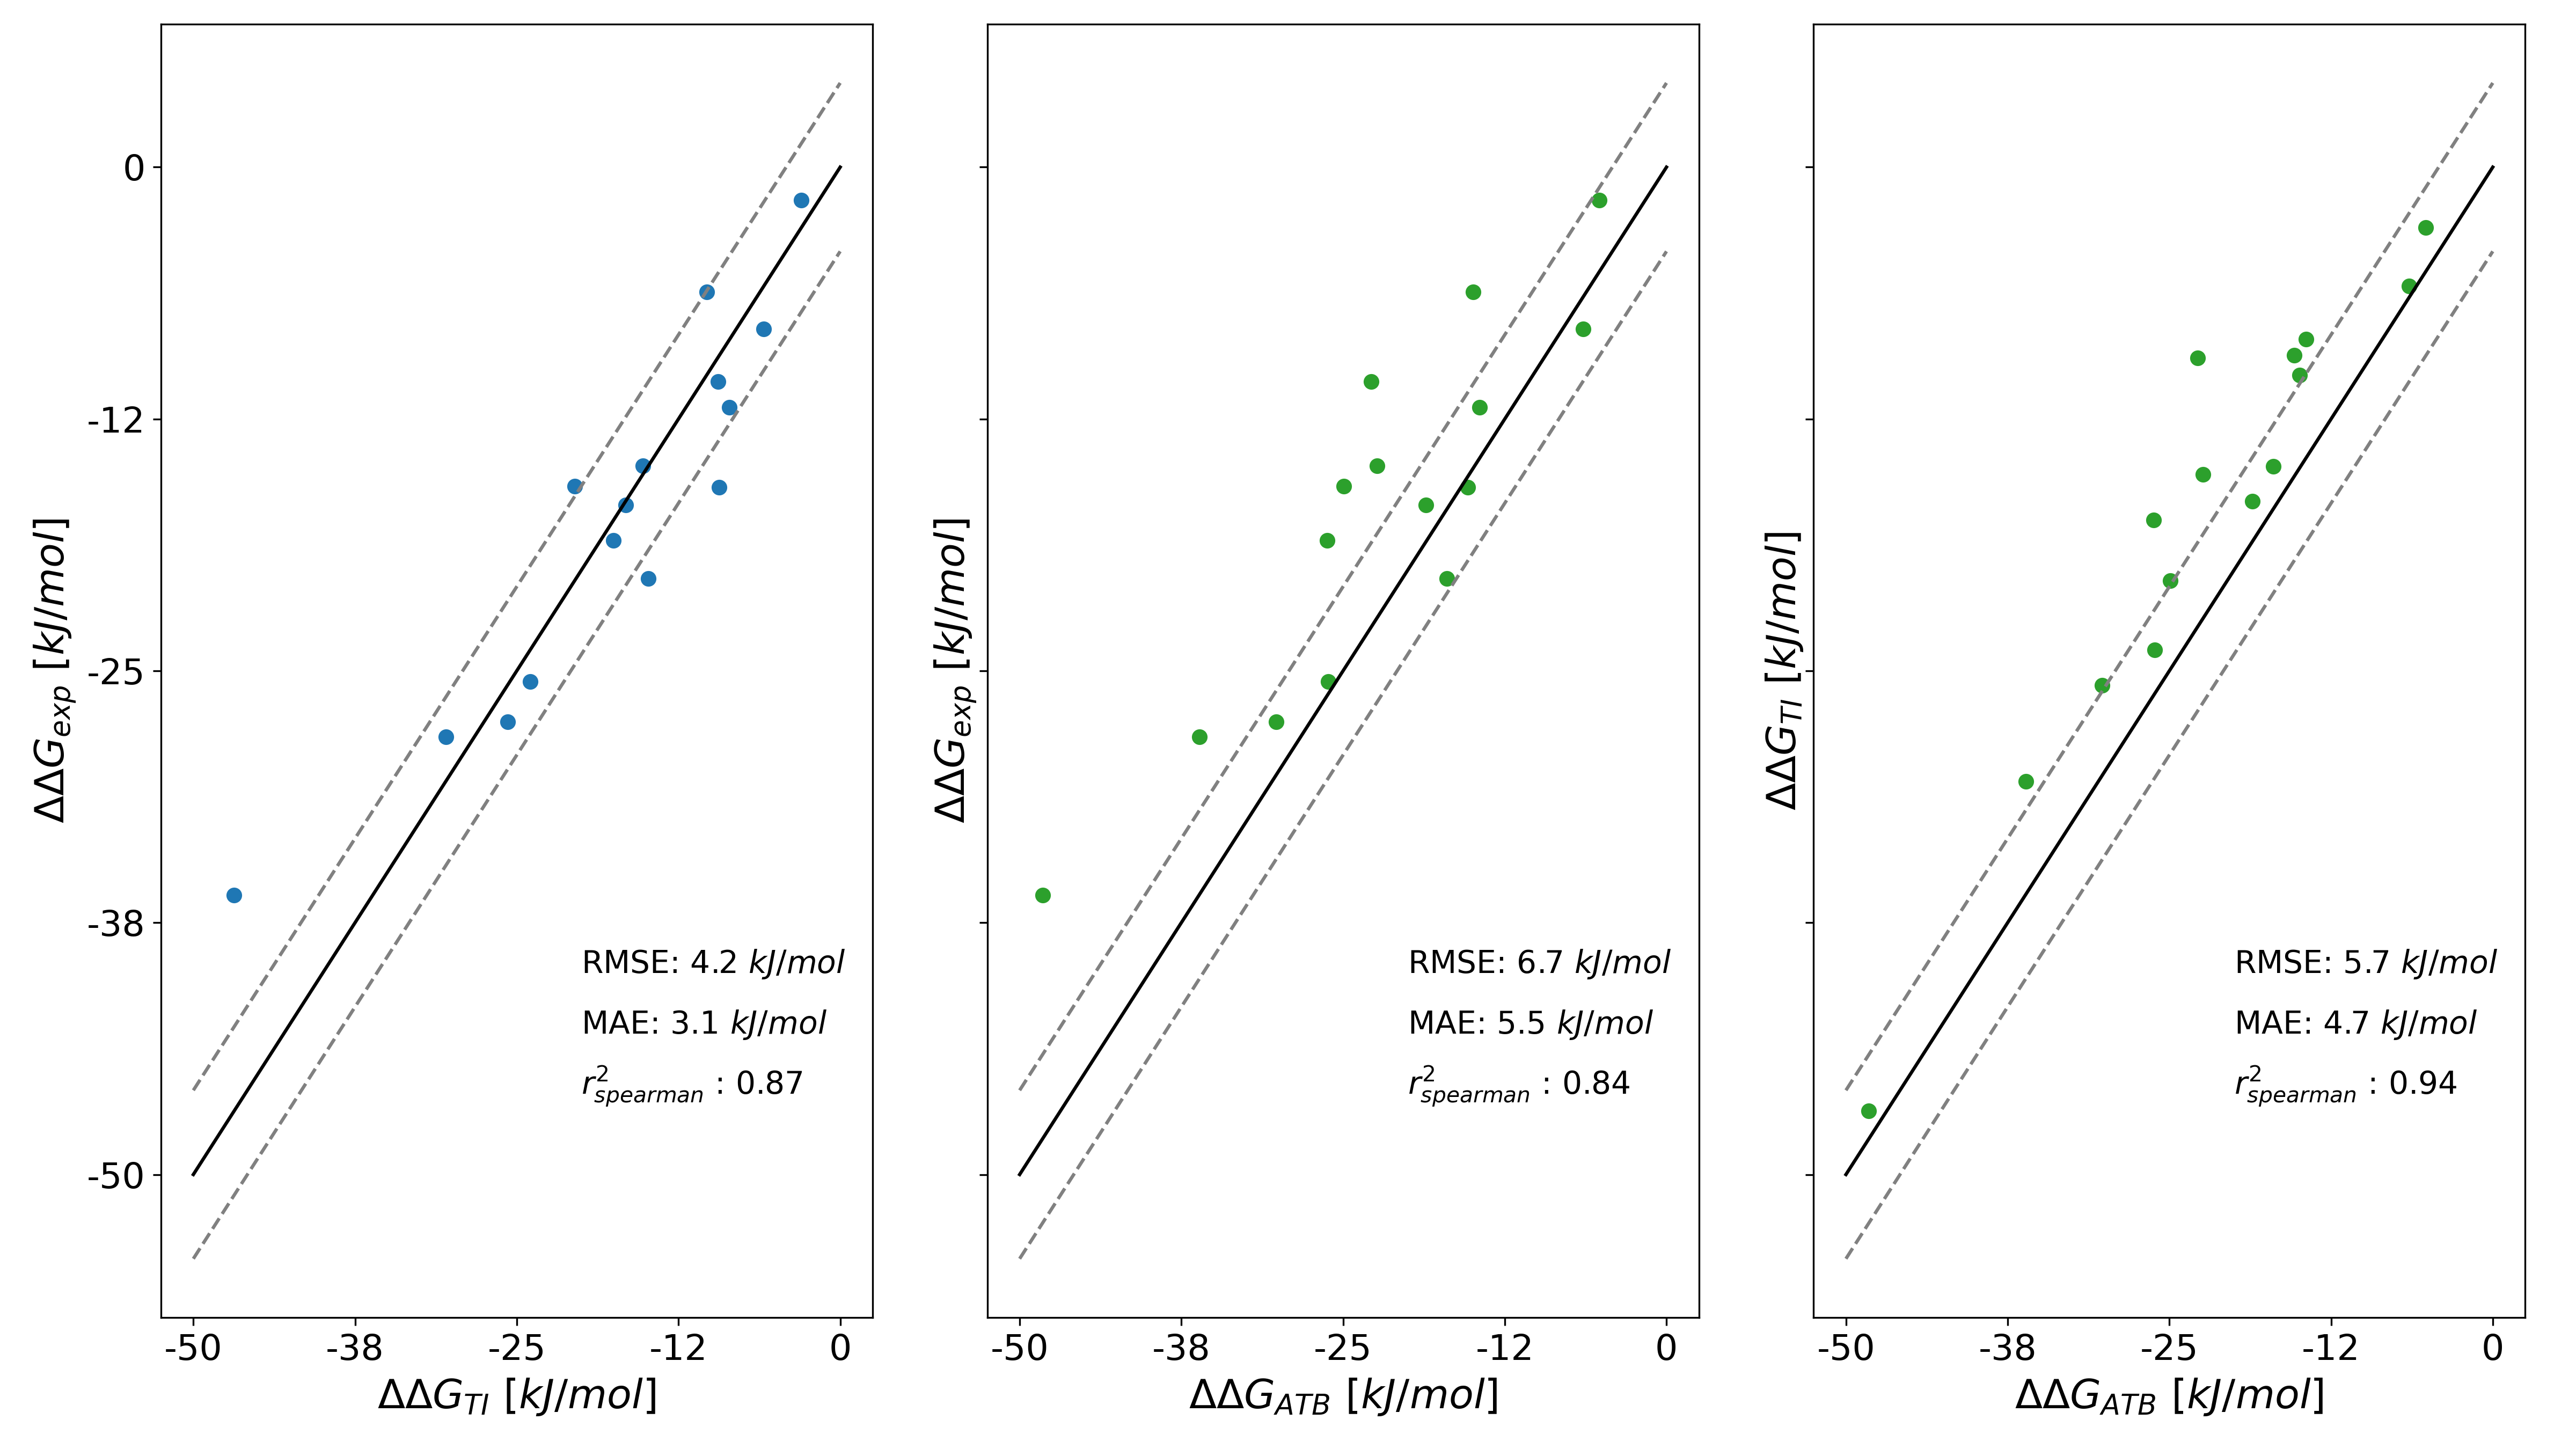
\includegraphics[width=\textwidth]{fig/results/pairwise/FE/M030_graph_ddG_solv_correlation_ATB_TI.png}
    \caption{Correlation of the different Calculation results for the pairwise TI-calculations.}
    \label{fig: pairCorr}
\end{figure}


\paragraph{Sampling}
%Coordinate analysis - Translation
The effect of the distance restraints on the system sampling behavior was studied further.
First, the translational fluctuations of the two aligned molecules were analyzed for each $\lambda$-window and molecule pair. For this, the pairwise distance of the COG of the restrained atoms in the rings was calculated. The Euclidean distance of both molecules' geometry centers fluctuates for $85\%$ of the simulation time maximally up to $0.0175$~nm from the average expected distance. Outlier distances (i.e. $5~\%$ of the simulation time) go up to maximally $0.0753$~nm for the pair of M030 and G209 and to $0.053$~nm for the molecule pair M030 and 8018. The other molecule pairs have outlier distances on average around $0.045$~nm. 
The results for the translational distance fluctuations show that the two molecule cores are well restrained to each other with the chosen distance restraints. (Fig. \ref{fig: pairCOGDist_TIStarMa})(Fig. \ref{fig: pairCOGDist_TIStarMa})

\begin{figure}[h]
    \centering
    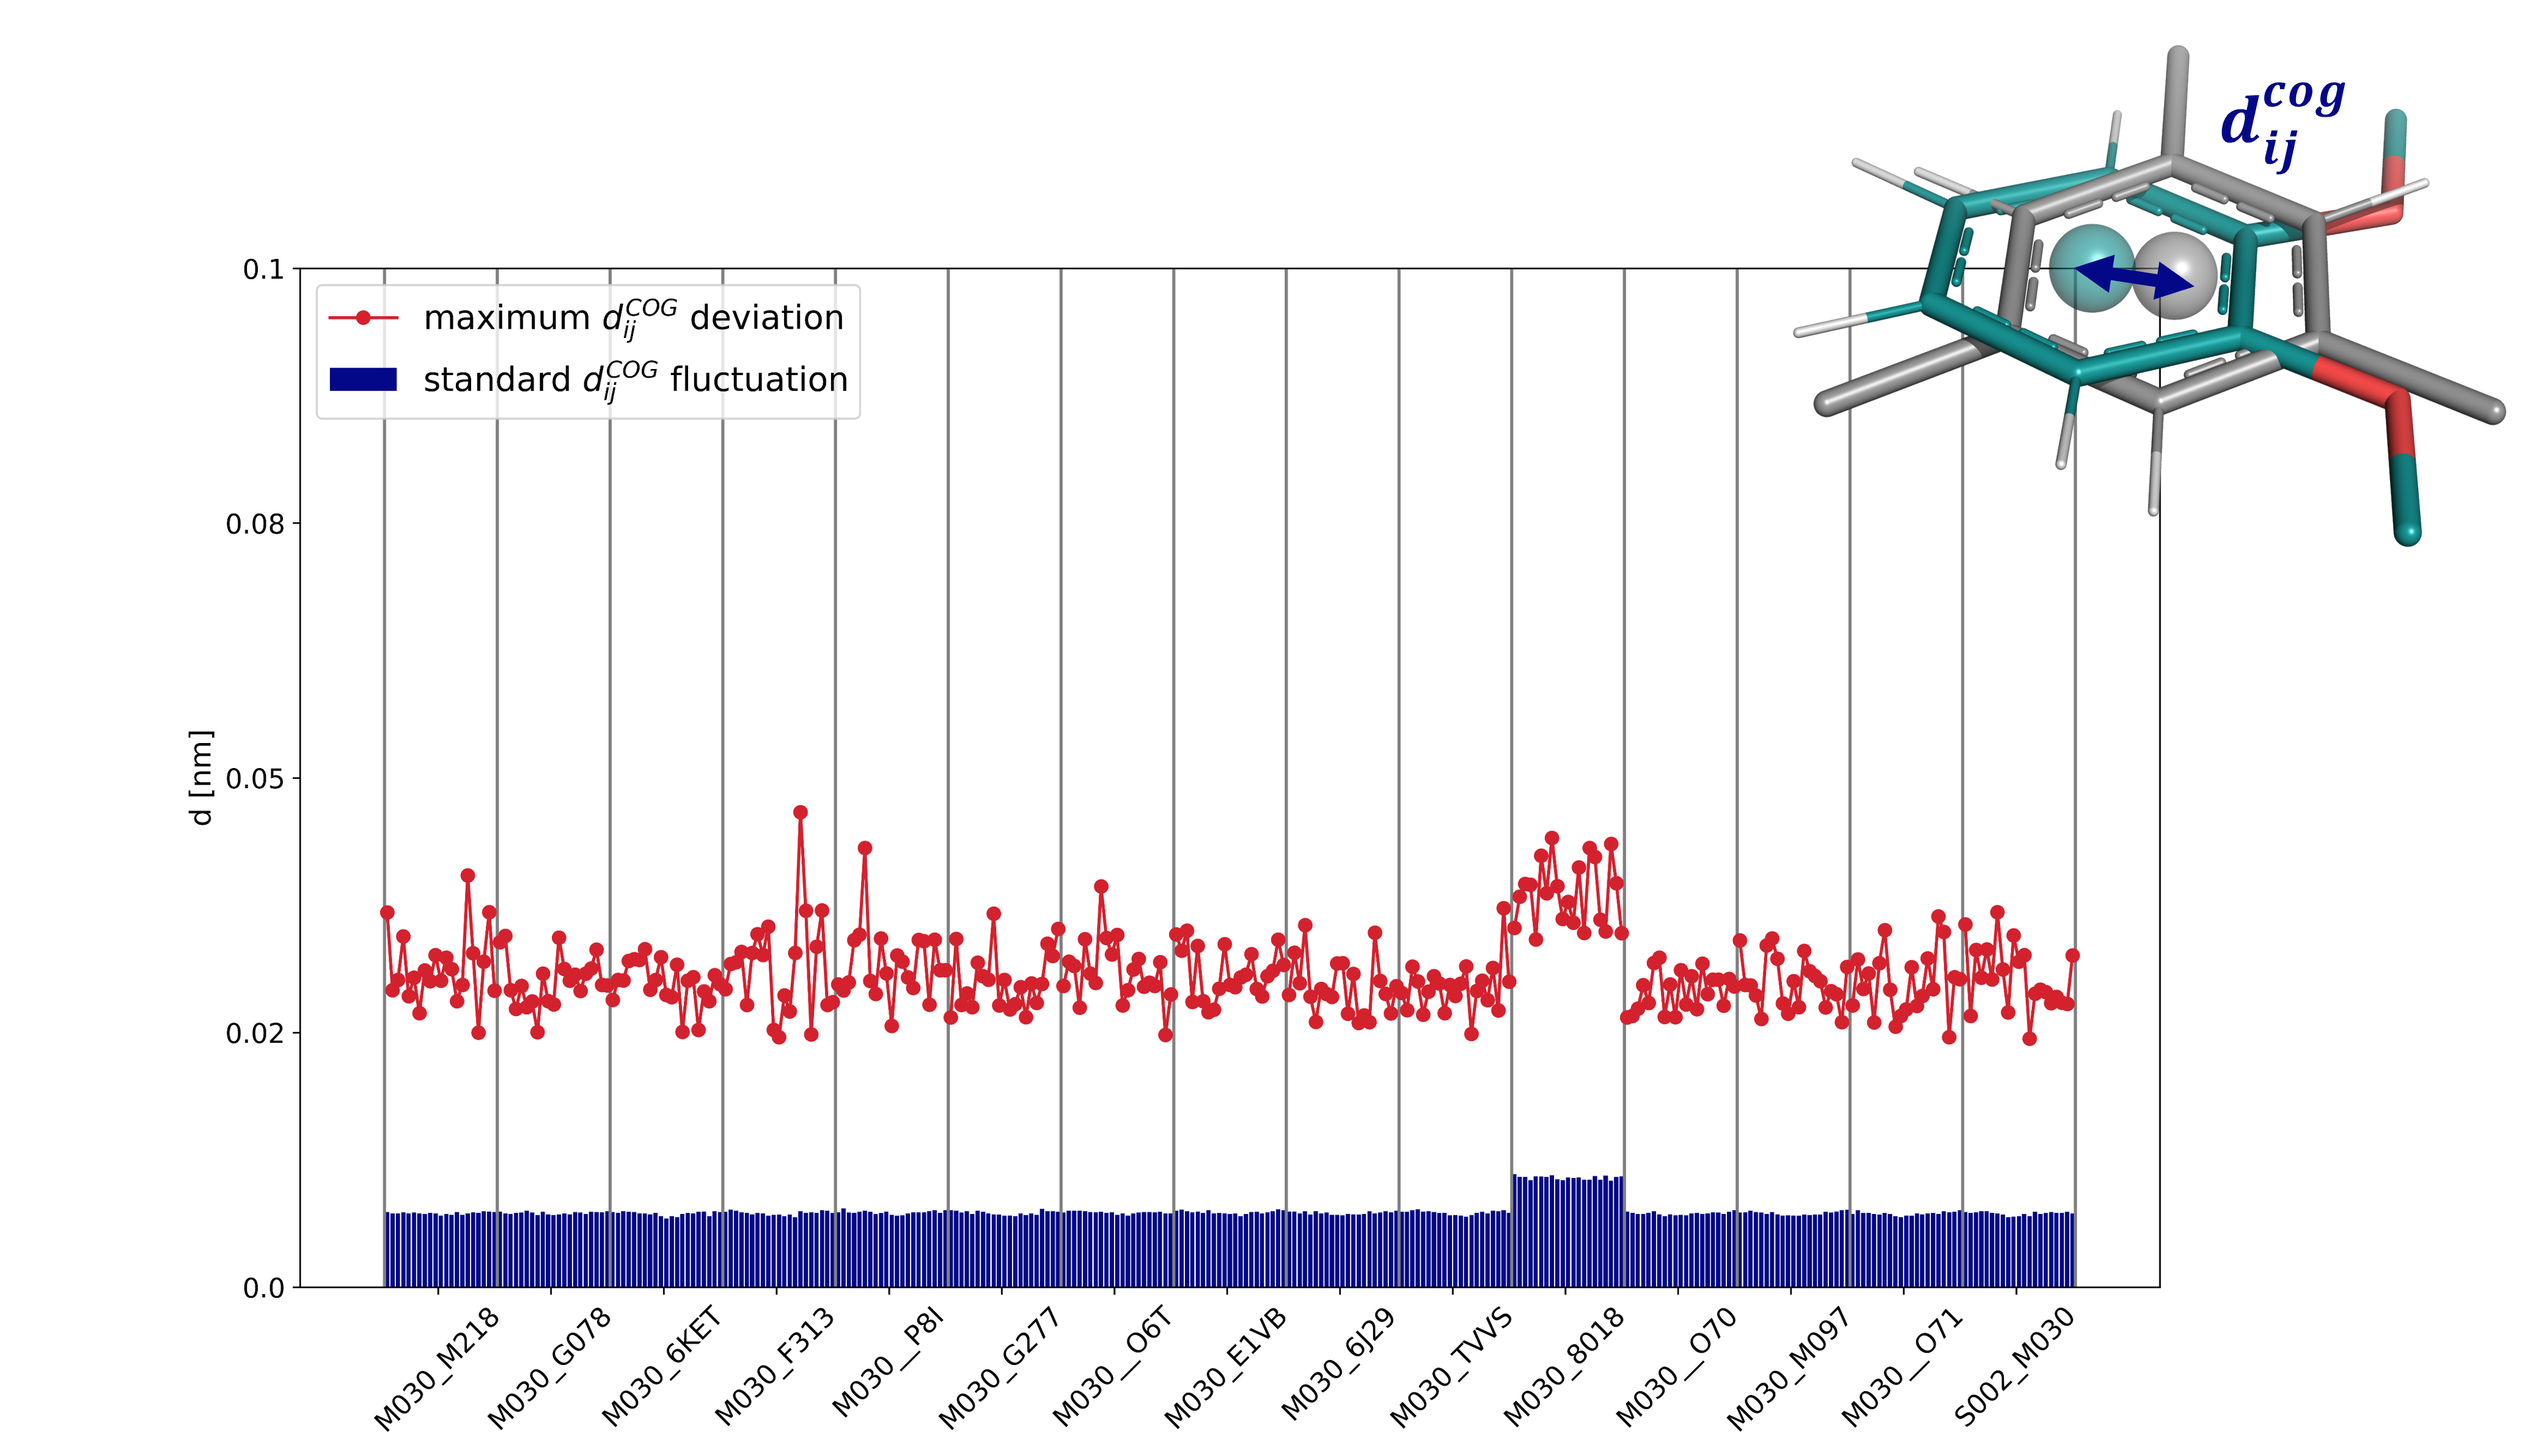
\includegraphics[width=\textwidth]{fig/results/pairwise/sampling/TI_pairwise_dCOG_fluctuations.png}
    \caption{Distribution of COG distances of both states during the simulations for the M030 pairwise TI-Graph. The COG was calculated for the restrained atoms in the rings. The x-axis for one molecule pair represents all the different $\lambda$ windows; i.e. $\lambda = 0$ to $\lambda = 1$. The molecules in the right upper corner are a schematic for the visualized effect.}
    \label{fig: pairCOGDist_TIStarMa}
\end{figure}

%Coordinate analysis - Rotation
Next, the rotation behavior of the restrained atoms in the molecule pairs was studied. For the relative rotation of the two molecules to each other, a maximal rotation of $6.3^\circ$ found. This rotation is a reasonably small rotation for one dimension. The ratio of rotations over $5.0^\circ$ occurring is for most pairs below $5\%$. This is with the exception of the M030 and \_O70 pair, where the flexible core ring of \_O70 leads to a slightly larger rotation frequency. The z-dimension of the molecule pairs in water shows significantly more minor deviations compared to the other dimensions. The required change can explain this for a rotation around the z-axis, which rotates the two molecules against each other in plane. In contrast, the x- and y-dimension rotation translates to a tilt of the molecules and is, therefore, easier accessible.  (Fig. \ref{fig: pairMolRotation_TIStarMap}).
 
 
\begin{figure}[h]
    \centering
    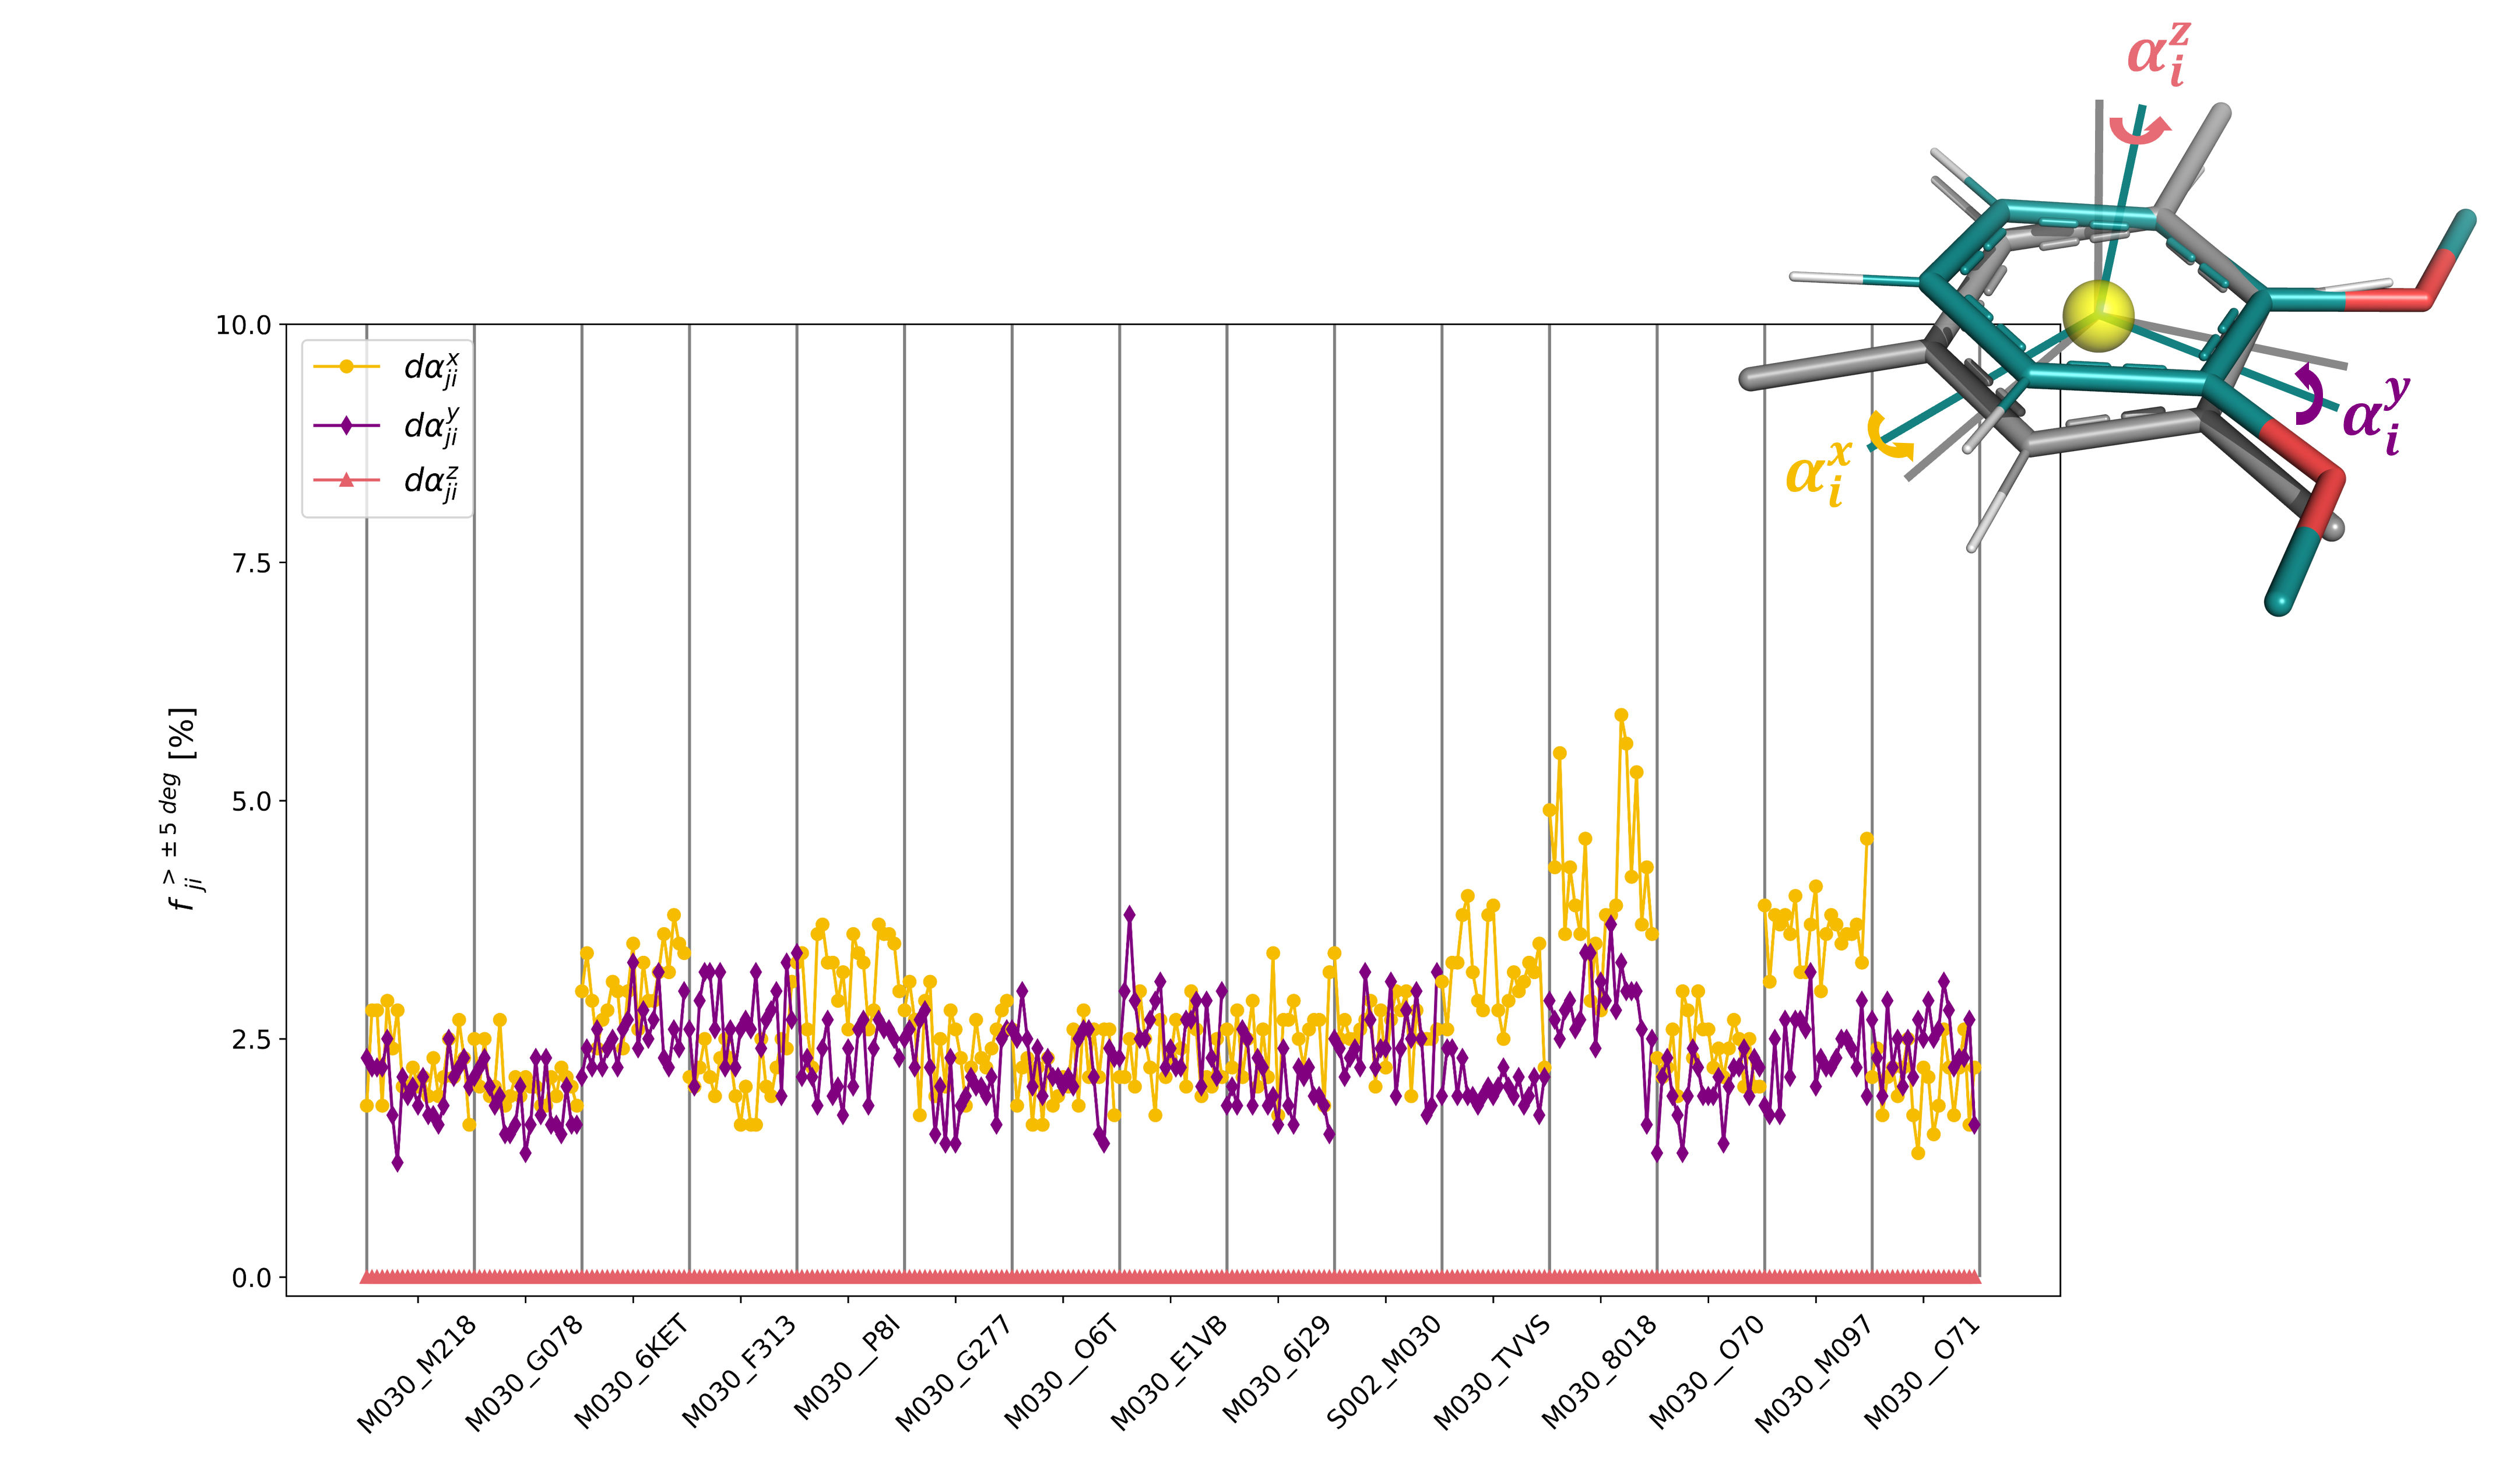
\includegraphics[width=\textwidth]{fig/results/pairwise/sampling/TI_pairwise_molecule_rotation.png}
    \caption{The figure shows the fraction of coordinates, in which the relative rotation of the two molecules to each other exceeds $5^{\circ}$.  The x-axis for one molecule pair represents all the different $\lambda$ windows; i.e. $\lambda = 0$ to $\lambda = 1$. The x-, y-, and z-axis were defined by the plane defined by the restrained atoms in each molecule. The molecules in the right upper corner are a schematic for the visualized effect. The z-axis rotation values were very small, as it translates to a rotation in plane, which is more difficult, than the tilt, that is introduced by rotation around the x- and y-axis. Therefore, the $f_{ji}$ for $d\alpha_{ji}^z$ is close to 0. }
    \label{fig: pairMolRotation_TIStarMap}
\end{figure}

%Torsion analysis:
A particular case in the free energy graph is calculating the relative hydration free energy of M030 and \_O70. This transition is of special interest, as the molecule \_O70 has a hexane core in contrast to the rigid benzene core of M030. The analysis of ring conformations was applied, originating from  \textit{Hansen et al.}.\cite{Hansen2010} The simulations of the physical states did not show any differences to single-molecule MD-simulations (Fig. \ref{SIfig: TIringTorisions}).

Additionally, the torsion angle sampling of the substituents of molecules F313, \_O6T, and 6KET were analyzed and compared to single-molecule MD-simulations. In this comparison, we could not see any differences in the sampling compared to the single state MD  (Fig. \ref{fig: TIsubsTorisions}). 

\begin{figure}[h]
    \centering
    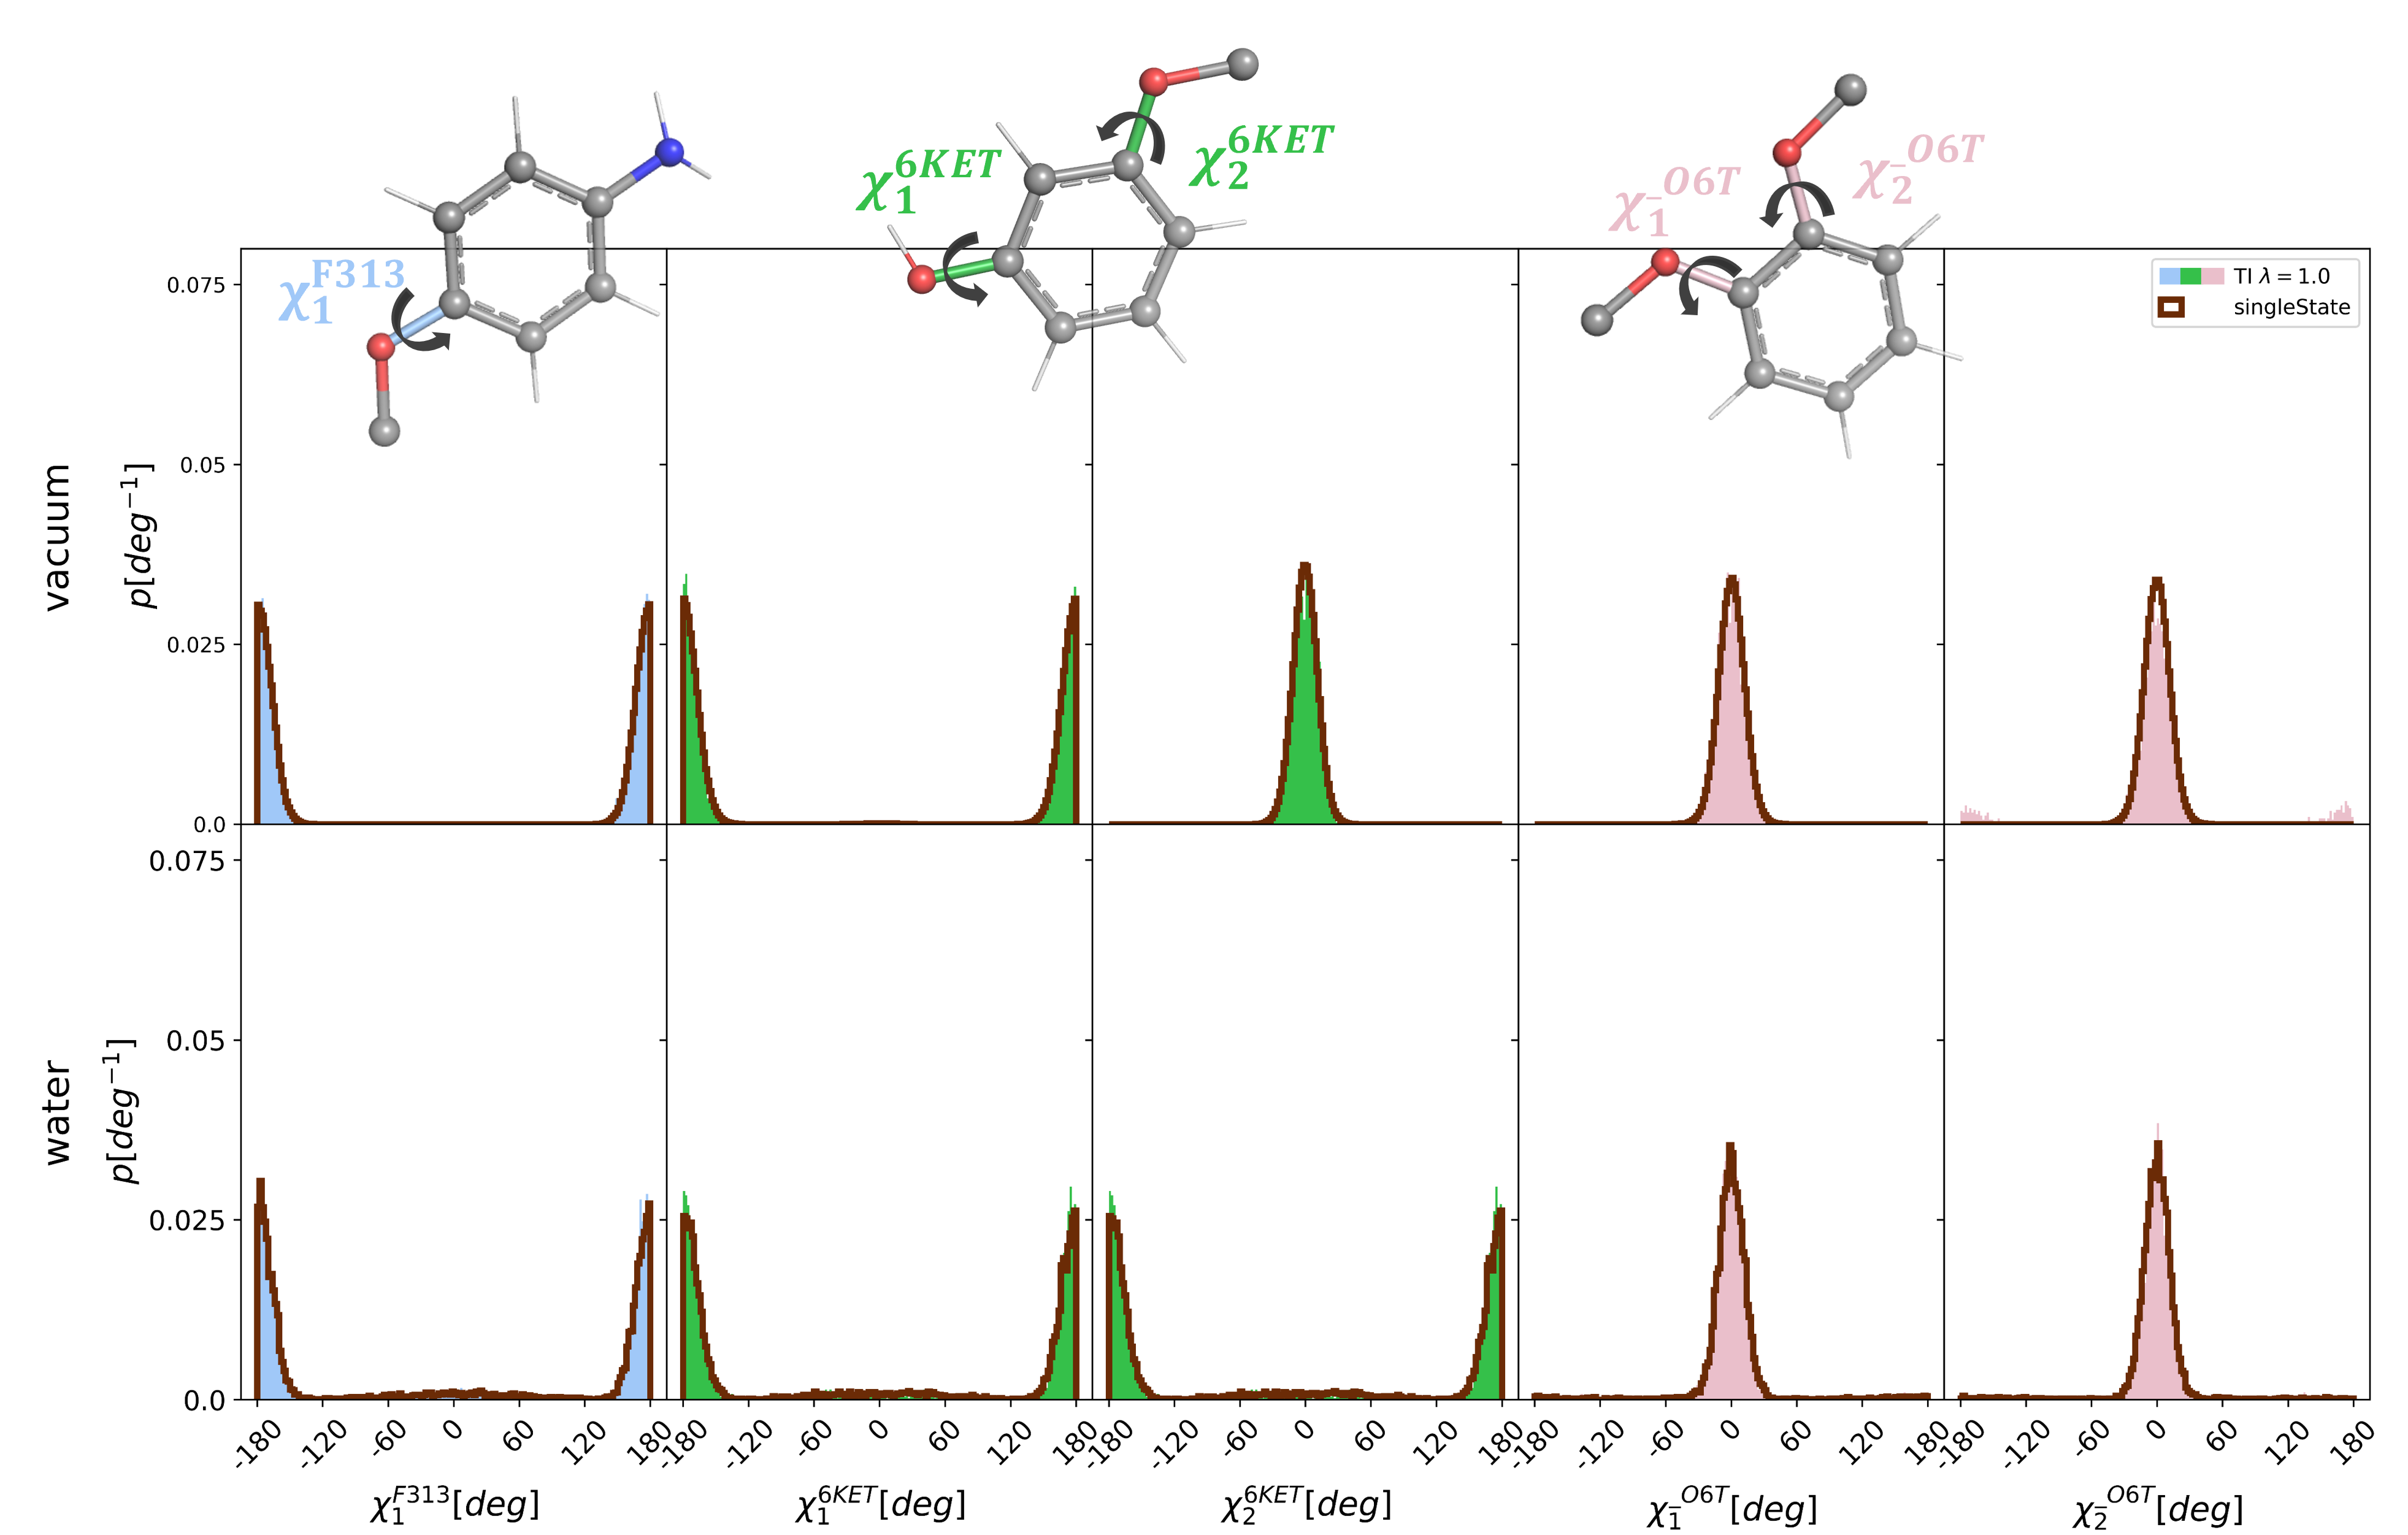
\includegraphics[width=\textwidth]{fig/results/pairwise/sampling/torsions/TI_all_substorsion_ana_partnerM030_singleState_populations_total.png}
    \caption{Normalized Distribution of Substituent torsion angles. The x-axis for one molecule pair represents all the different $\lambda$ windows; i.e. $\lambda = 0$ to $\lambda = 1$.  The molecules in the right upper corner are a schematic for the visualized effect.}
    \label{fig: TIsubsTorisions}
\end{figure}



\begin{table}[H]
\caption{Hydration free energy statistics comparison. This table shows a comparison of the RMSE and MAE, the Spearman correlation, as well as the used simulation time for the preparation and production of the different simulation methods. For TI and RE-EDS, relative hydration free energies were calculated, whereas for ATB, absolute hydration free energies are reported. The relative hydration free energies were then calculated as the pairwise difference of the reported absolute hydration free energies. For the TI simulations of set A, all pairwise free energy differences were calculated. For the TI simulations of set B, only 9 pairwise free energy differences were calculated and the remaining 36 were calculated as pairwise differences. The uncertainty for the RMSE values was estimated by a 100 times iterated bootstrap approach.}
\label{tab:Benz_set2_Eoff}
\resizebox{\columnwidth}{!}{%
\centering
\begin{tabular}{ l | c | c  | c |c c | c |c c | }
 Metric & \multicolumn{2}{c|}{pairwise}&\multicolumn{6}{c|}{multistate}  \\ 
        & \multicolumn{2}{c|}{}        & \multicolumn{3}{c|}{setA} & \multicolumn{3}{c|}{setB}  \\ 
        & absolute & relative          & absolute & \multicolumn{2}{c|}{relative} & absolute &  \multicolumn{2}{c|}{relative}\\ 
  & ATB & TI & ATB & TI & RE-EDS & ATB & TI & RE-EDS\\ 
 \hline
    RMSE~$[\mathrm{kJ/mol}]$ & $6.7 ~\pm~ 0.3$ & $4.2 ~\pm~ 0.3$ & $6.2 ~\pm~ 0.3$ & $3.7 ~\pm~ 0.1$ & $3.6 ~\pm~ 0.3$ & $5.8 ~\pm~ 0.1$ & $3.4 ~\pm~ 0.1$ & $3.3 ~\pm~ 0.1$ \\ 
    MAE~$[\mathrm{kJ/mol}]$ & $5.5$ $\pm$ $3.9$ & $3.1$ $\pm$ $2.7$ & $5.3$ $\pm$ $3.2$ & $3.0$ $\pm$ $2.1$ & $3.0$ $\pm$ $2.2$ & $4.8$ $\pm$ $3.3$ & $2.8$ $\pm$ $2.0$ & $2.7$ $\pm$ $1.8$ \\ 
    $\mathrm{r}^2_{\mathrm{spearman}}$ & $0.84$ & $0.87$ & $0.92$ & $0.93$ & $0.93$ & $0.93$ & $0.96$ & $0.96$ \\
    $\mathrm{t}_{\mathrm{preparation}}~[\mathrm{ns}]$ & & $630$ & $-$ & $215$ & $222$ & $-$ &   $378$ & $418$ \\
    $\mathrm{t}_{\mathrm{production}}~[\mathrm{ns}]$ &  & $3150$ & $-$ & $1050$ & $36$  & $-$ & $1890$ & $212$ \\
\end{tabular}
}
\end{table}


%================================================================================
%\appsection[CBTI and Quadrature]{quad}{Relationship between CBTI and Quadrature Integration}
%================================================================================



\section{Ligands}
\begin{center}
%\scriptsize
\resizebox{\columnwidth}{!}{%
\begin{tabular}{l | l | l}
ligand & IUPAC name & canonical SMILES (Daylight)\\
\hline
\_O6T & 1,2-Dimethoxybenzene & COc1ccccc1OC \\
\_O70 & (2R,5R)-2-methyl-5-prop-1-en-2-ylcyclohexan-1-one & CC(=C)[C@@H]1CC[C@H](C(=O)C1)C\\
\_O71 & (1S,5R)-2-methyl-5-prop-1-en-2-ylcyclohex-2-en-1-ol & CC(=C)[C@@H]1CC=C([C@H](C1)O)C\\ 
\_P8I & Cyclopentanone & O=C1CCCC1\\
6J29 & 1-amino-4-hydroxyanthracene-9,10-dione & Oc1ccc(c2c1C(=O)c1ccccc1C2=O)N\\
6KET & 3-Methoxyphenol & COc1cccc(c1)O\\
8018 & - & Cl[C@@H]1C[C@H]2[C@@H]([C@H]1Cl)[C@]1(C([C@]2(Cl)C(=C1Cl)Cl)(Cl)Cl)Cl\\
E1VB & - & F[C@H](C(F)F)Oc1ccccc1\\
F313 & 4-Methoxyaniline & COc1ccc(cc1)N\\
G078 & 1,4-Dimethylnaphthalene & Cc1ccc(c2c1cccc2)C\\
G277 & cyclohexa-2,5-diene-1,4-dione & O=C1C=CC(=O)C=C1\\
M030 & 1,3,5-Trimethylbenzene & Cc1cc(C)cc(c1)C\\
M097 & 2-Chloroaniline & Nc1ccccc1Cl\\
M218 & N-Methylaniline & CNc1ccccc1 \\
S002 & - & BrCc1ccccc1\\
TVVS & - & O=CC1=CC=[N]=CC1 \\
\end{tabular}
}
\end{center}

\section{Restraint Placement}
\begin{figure}
    \centering
    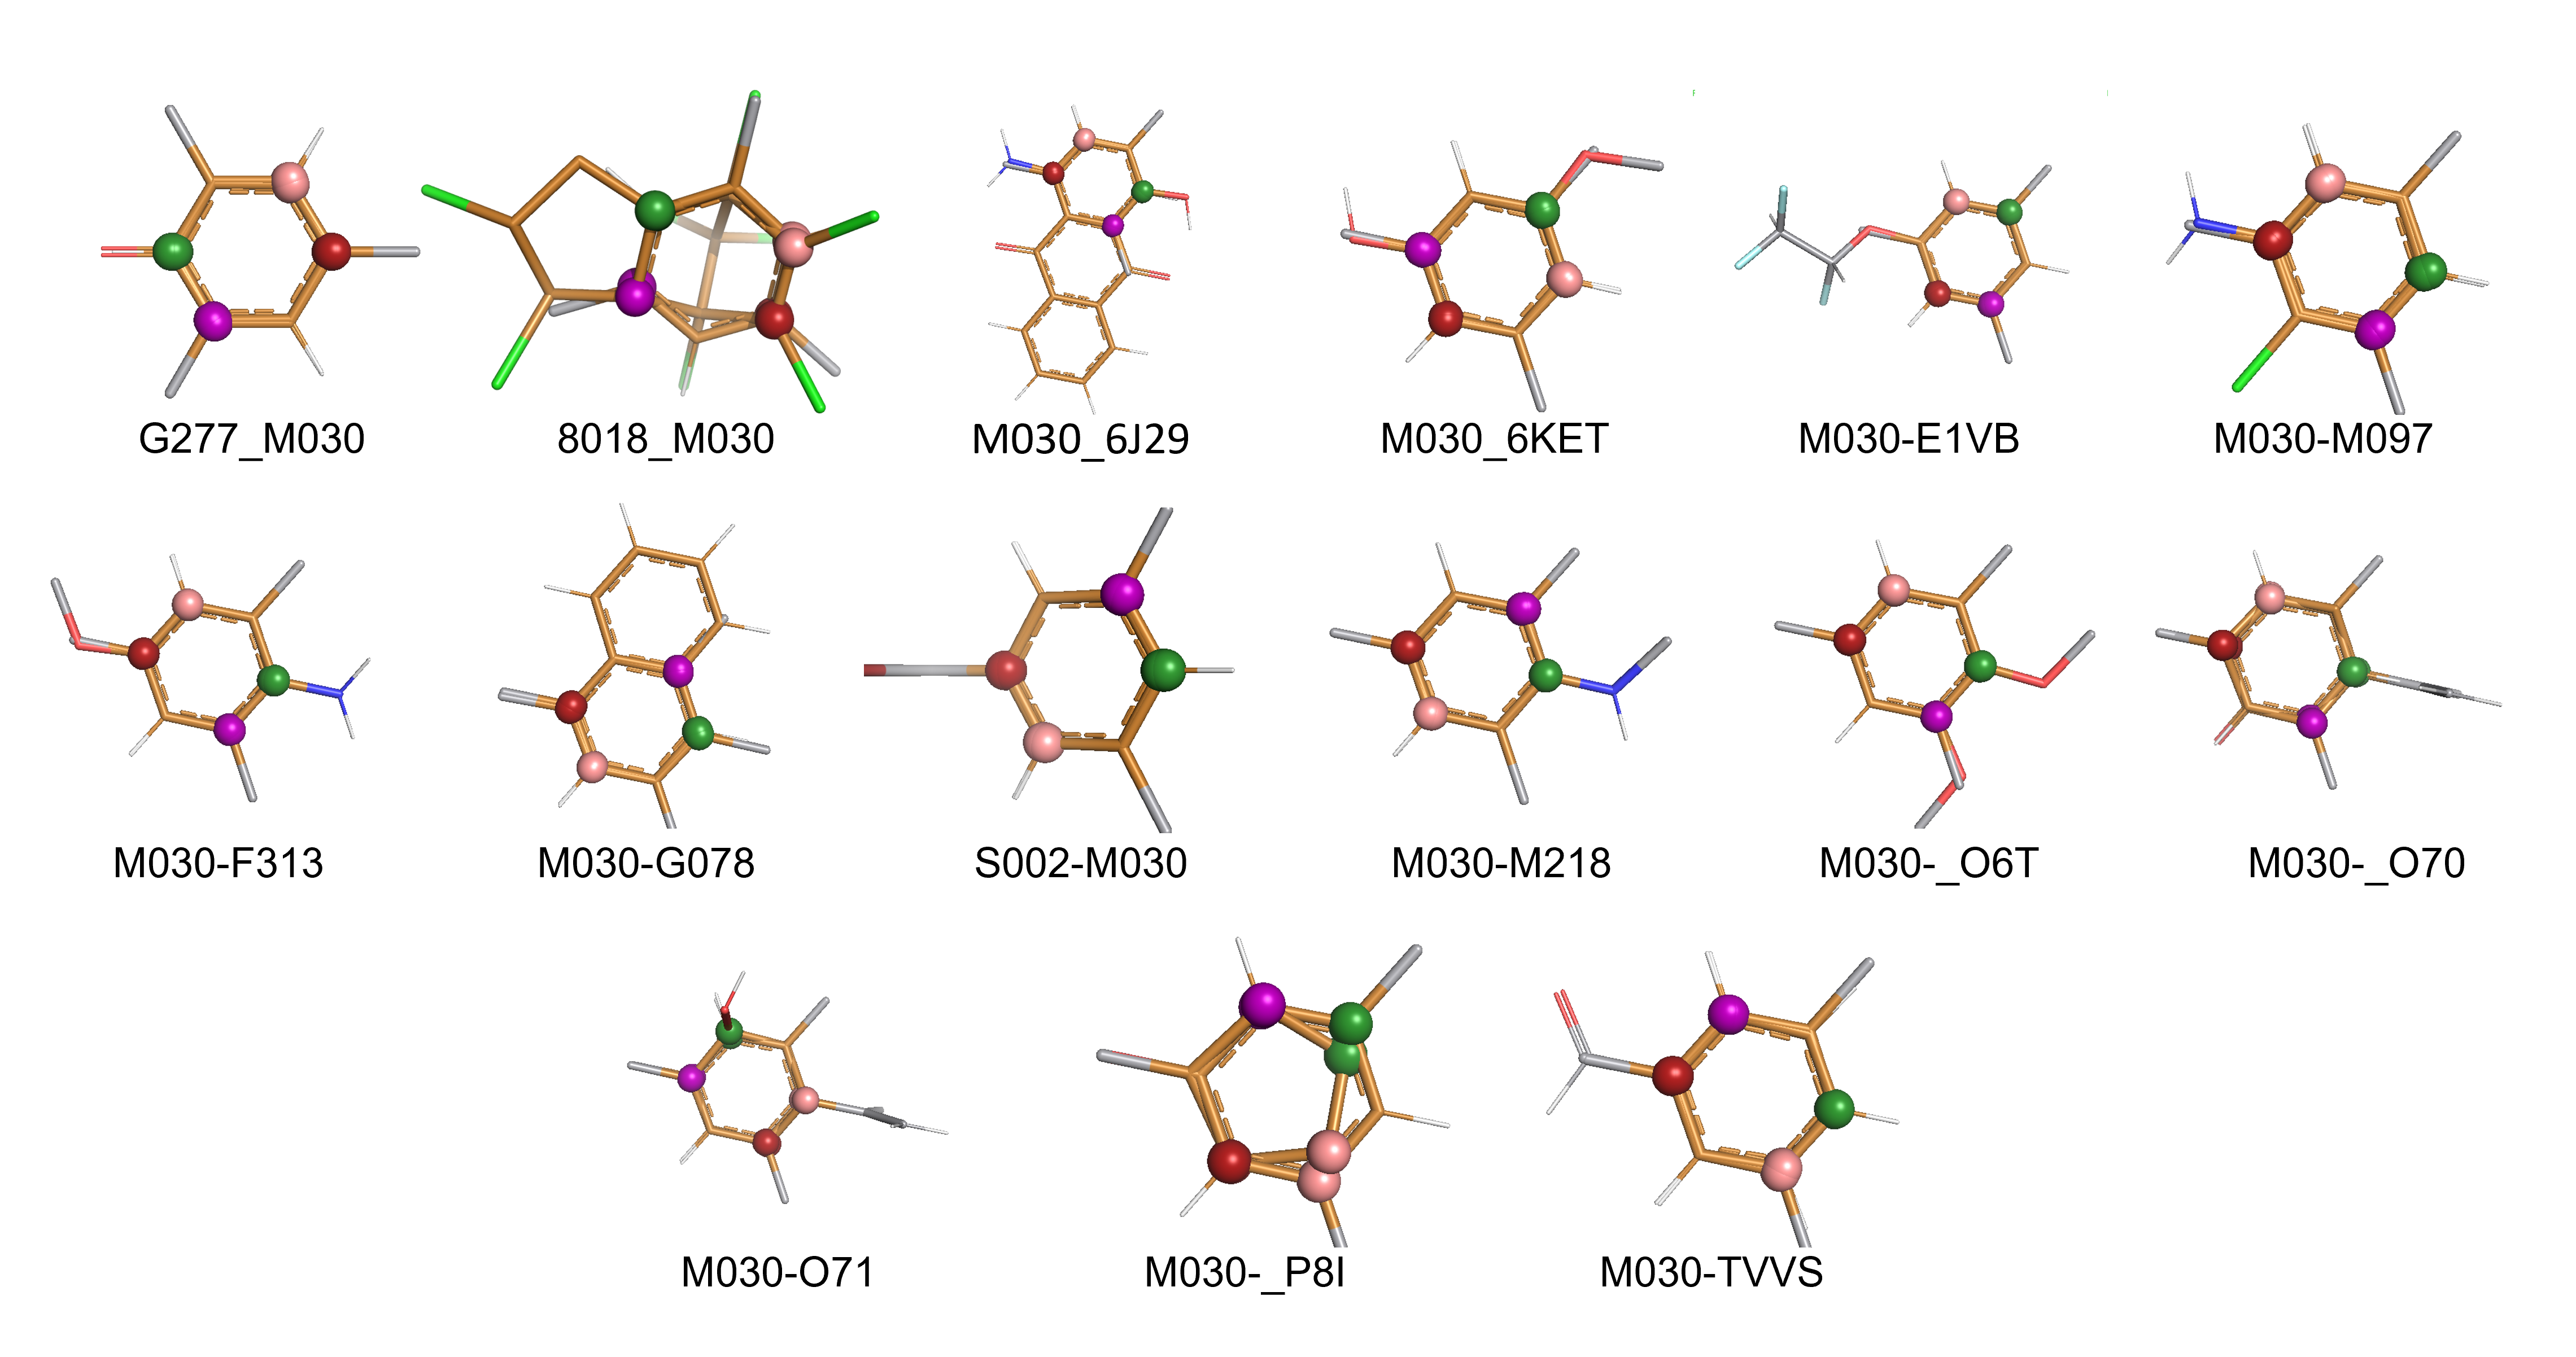
\includegraphics[width=\textwidth]{fig/results/pairwise/restraintPlacement/Restraints_PairwiseTI_M030Graph.png}
    \caption{Placement of the restraints for the pairwise TI- M030 system}
    \label{SIfig: Pairwise_TI_M030_Graph}
\end{figure}

\begin{figure}
    \centering
    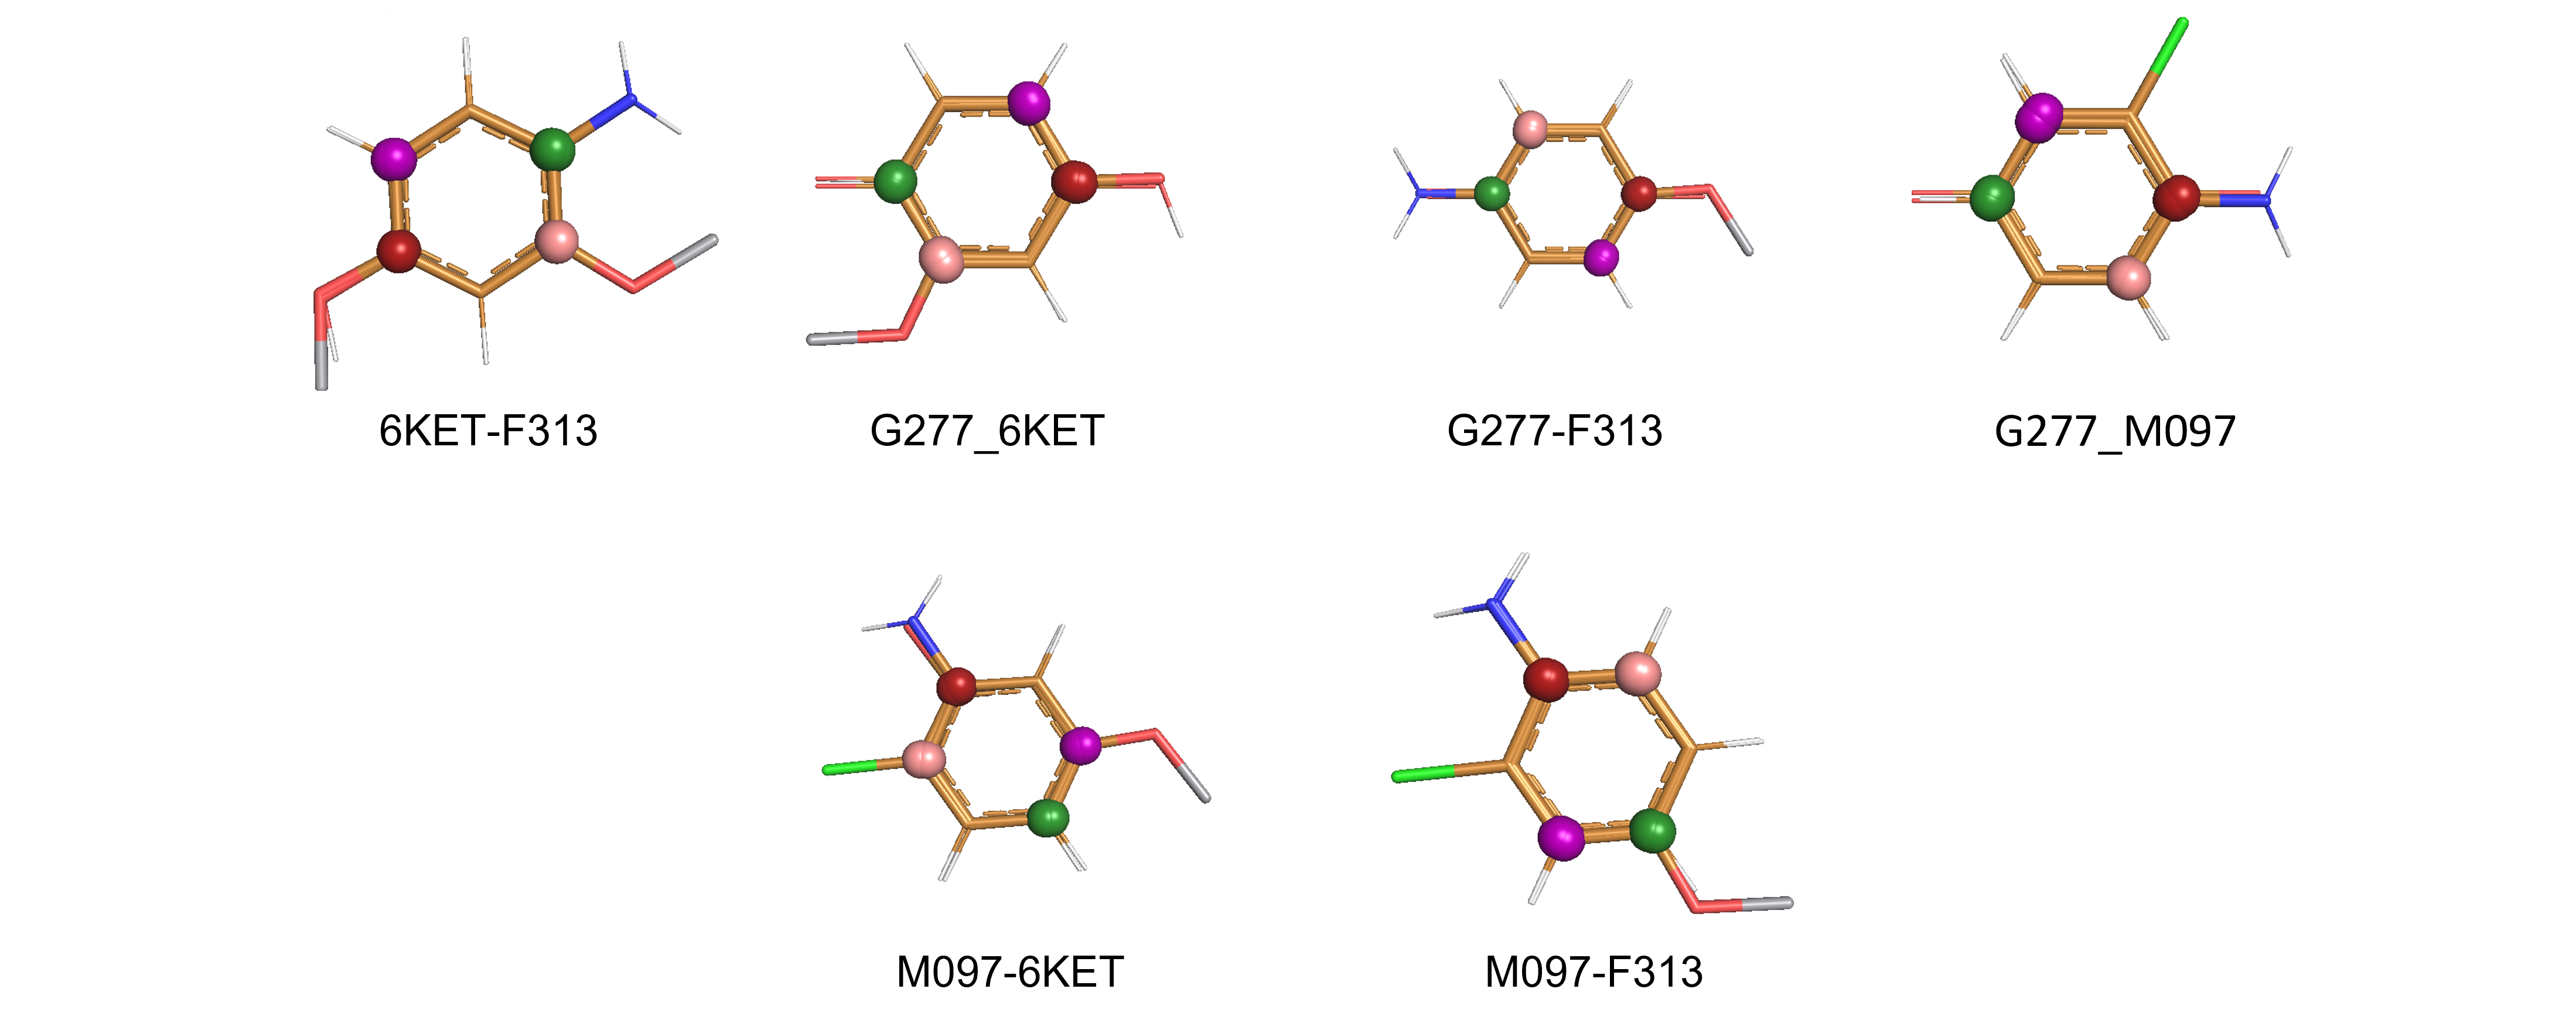
\includegraphics[width=\textwidth]{fig/results/pairwise/restraintPlacement/Restraints_PairwiseTI_reedsaddition.png}
    \caption{Placement of the restraints for the TI calculation for the full graph comparison to multistate set A}
    \label{SIfig:Pairwise_TI_AddRE-EDS_Graph}
\end{figure}

\clearpage

\section{Relative Hydration Free Energy Calculations}
\subsection{Pairwise TI}

\begin{table}[H]
\caption{Pairwise relative hydration free energies with one base molecule. Experimental data and the ABFE calculations by ATB are taken from the ATB database.\cite{Martin2018} The RAFE was calculated from the experimental and the ABFE ATB  data. The RAFE results of the TI approach use the introduced restraint approach. The uncertainty was calculated via Gaussian error propagation of the provided errors. The experimental uncertainty for the pair G277-M030 could not be provided, as the experimental uncertainty of G277 is not provided in the ATB database. The RMSE and its uncertainty were estimated with a 100 fold bootstrap approach.}
\begin{center}
%\resizebox{\columnwidth}{!}{%
\footnotesize
\begin{tabular}{ c c |c |c|c|}
  \multicolumn{2}{c|}{Ligands} & \multicolumn{1}{c|}{Experiment} &\multicolumn{1}{c|}{ATB}&\multicolumn{1}{c|}{TI}\\ 
    $i$ & $j$ & [kJ~mol$^{-1}$] & [kJ~mol$^{-1}$] & [kJ~mol$^{-1}$]  \\
  \hline
        \_O6T &  M030 &  $18.5 ~\pm~ 1.3$  &  $26.2 ~\pm~ 0.8$ &  $  17.5 ~\pm~ 0.7$\\
        \_O70 &  M030 &  $11.9 ~\pm~ 1.3$  &  $14.4 ~\pm~ 0.7$ &  $  8.6 ~\pm~ 0.6 $\\
        \_O71 &  M030 &  $14.8 ~\pm~ 1.5$  &  $22.4 ~\pm~ 0.7$ &  $ 15.2 ~\pm~ 0.9 $\\
        \_P8I &  M030 &  $15.9 ~\pm~ 1.8$  &  $15.3 ~\pm~ 0.6$ &  $  9.4 ~\pm~ 0.4 $\\
        6J29 &  M030 &   $36.1 ~\pm~ 1.4$  &  $48.2 ~\pm~ 0.4$ &  $ 46.9 ~\pm~ 0.8 $\\
        6KET &  M030 &   $28.1 ~\pm~ 1.8$  &  $36.1 ~\pm~ 0.6$ & $  30.5 ~\pm~ 0.5 $\\
        8018 &  M030 &   $10.6 ~\pm~ 1.3$  &  $22.8 ~\pm~ 0.5$ &  $  9.5 ~\pm~ 0.9 $\\
        E1VB &  M030 &   $ 1.6 ~\pm~ 1.8$  &  $ 5.2 ~\pm~ 0.7$ &  $ 3.0 ~\pm~ 1.2 $\\
        F313 &  M030 &   $27.5 ~\pm~ 1.8$  &  $30.2 ~\pm~ 0.6$ &  $ 25.7 ~\pm~ 0.5 $\\
        G078 &  M030 &   $ 8.0 ~\pm~ 1.8$  &  $ 6.5 ~\pm~ 0.6$ &  $  5.9 ~\pm~ 0.5 $\\
        G277 &  M030 &   $20.4 $           &  $17.0 ~\pm~ 0.6$ &  $ 14.8 ~\pm~ 0.39 $\\
        M030 &  M097 &   $16.8 ~\pm~ 1.8$  &  $18.6 ~\pm~ 0.6$ &  $ 16.6 ~\pm~ 0.5 $\\
        M030 &  M218 &   $15.9 ~\pm~ 1.8$  &  $24.9 ~\pm~ 0.6$ &  $ 20.5 ~\pm~ 0.5 $\\
        M030 &  S002 &    $6.2 ~\pm~ 1.3$  &  $14.9 ~\pm~ 0.7$ &  $ 10.3 ~\pm~ 0.4 $\\
        M030 &  TVVS &   $25.5 ~\pm~ 1.8$  &  $26.1 ~\pm~ 0.6$ &   $ 24.0 ~\pm~ 0.4 $\\
  \hline
        \multicolumn{2}{c|}{RMSE} &          & $6.7 ~\pm~ 0.3$ & $4.2 ~\pm~ 0.3 $\\
        \multicolumn{2}{c|}{MAE} &           & $5.5 ~\pm~ 3.9$ & $3.1 ~\pm~ 2.7$ \\
        %\multicolumn{2}{c|}{$r^2_{\text{Pearson}}$} & & 0.90  & 0.93 \\
        \multicolumn{2}{c|}{$r^2_{\text{Spearman}}$} &  & $0.84$ & $0.87$  \\
        \multicolumn{2}{c|}{$t_{preparation}$} & & &  $630$~ns \\
        \multicolumn{2}{c|}{$t_{production}$} & & &  $3150$~ns \\
    % ABFE scale nonbondes, such that mol vanishes.
%ATB: inital: 11 lams * 2envs*(vac: 1.0ns + 1ns/ solv: 0.5ns+0.5ns) when error not below 0.5kJ (on Homepage 1.5kJ....)
%               min = 66*15 = 990ns minimal!
%   max?:  18 lams * 2envs*(vac: 1.0ns + 1ns/ solv: 0.5ns+0.5ns) when error not below 0.5kJ (on Homepage 1.5kJ....)
%               max = 66*15 = 1620ns max!
% average: 15 lams * 2envs*(vac: 1.0ns + 1ns/ solv: 0.5ns+0.5ns) when error not below 0.5kJ
%               avg = 66*15 = 1350ns avg!
%TI:
% 15edges*21lam*5ns*2envs = 3150 ns / 1890ns (3ns)
%TI-eq:
% 15edges*21lam*1ns*2envs = 630 ns
\end{tabular}
%}
\end{center}
\label{SITab: FE_M030_Graph}
\end{table}

\begin{figure}
    \centering
    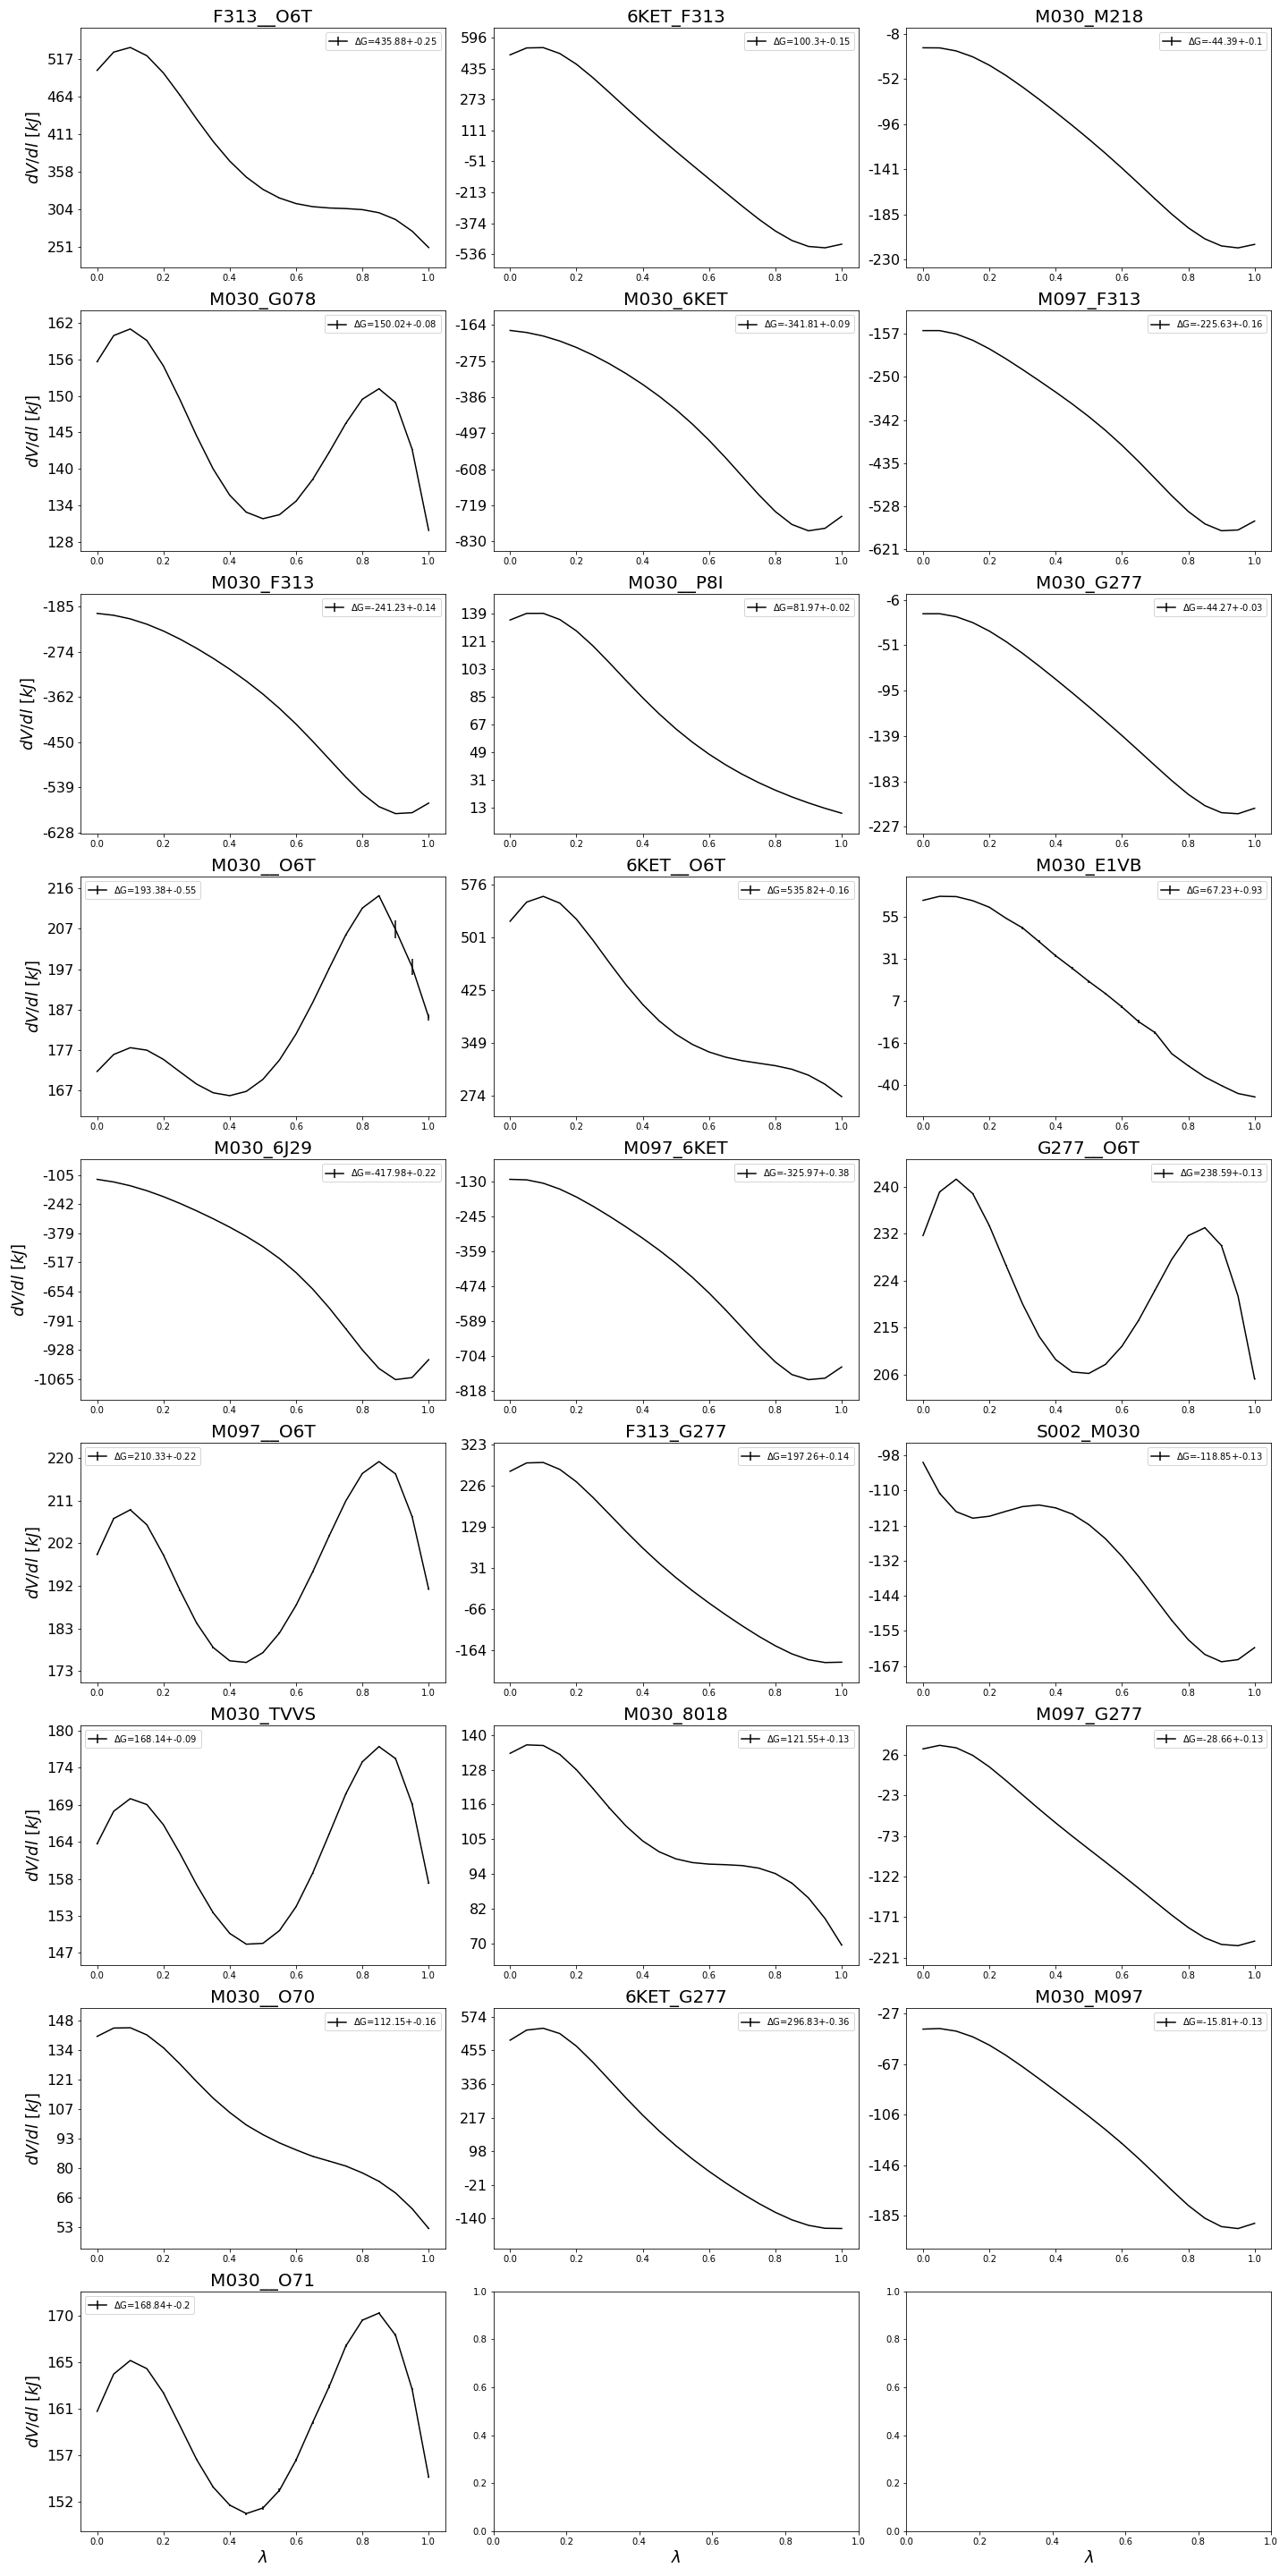
\includegraphics[width=0.65\textwidth]{fig/SI/dG_convergence/TI_vacuum_lambda_curves.png}
    \caption{Pairwise TI-Vacuum $\lambda$-curves}
    \label{SIfig:TI_vacuum_curve}
    \end{figure}

\begin{figure}
    \centering
    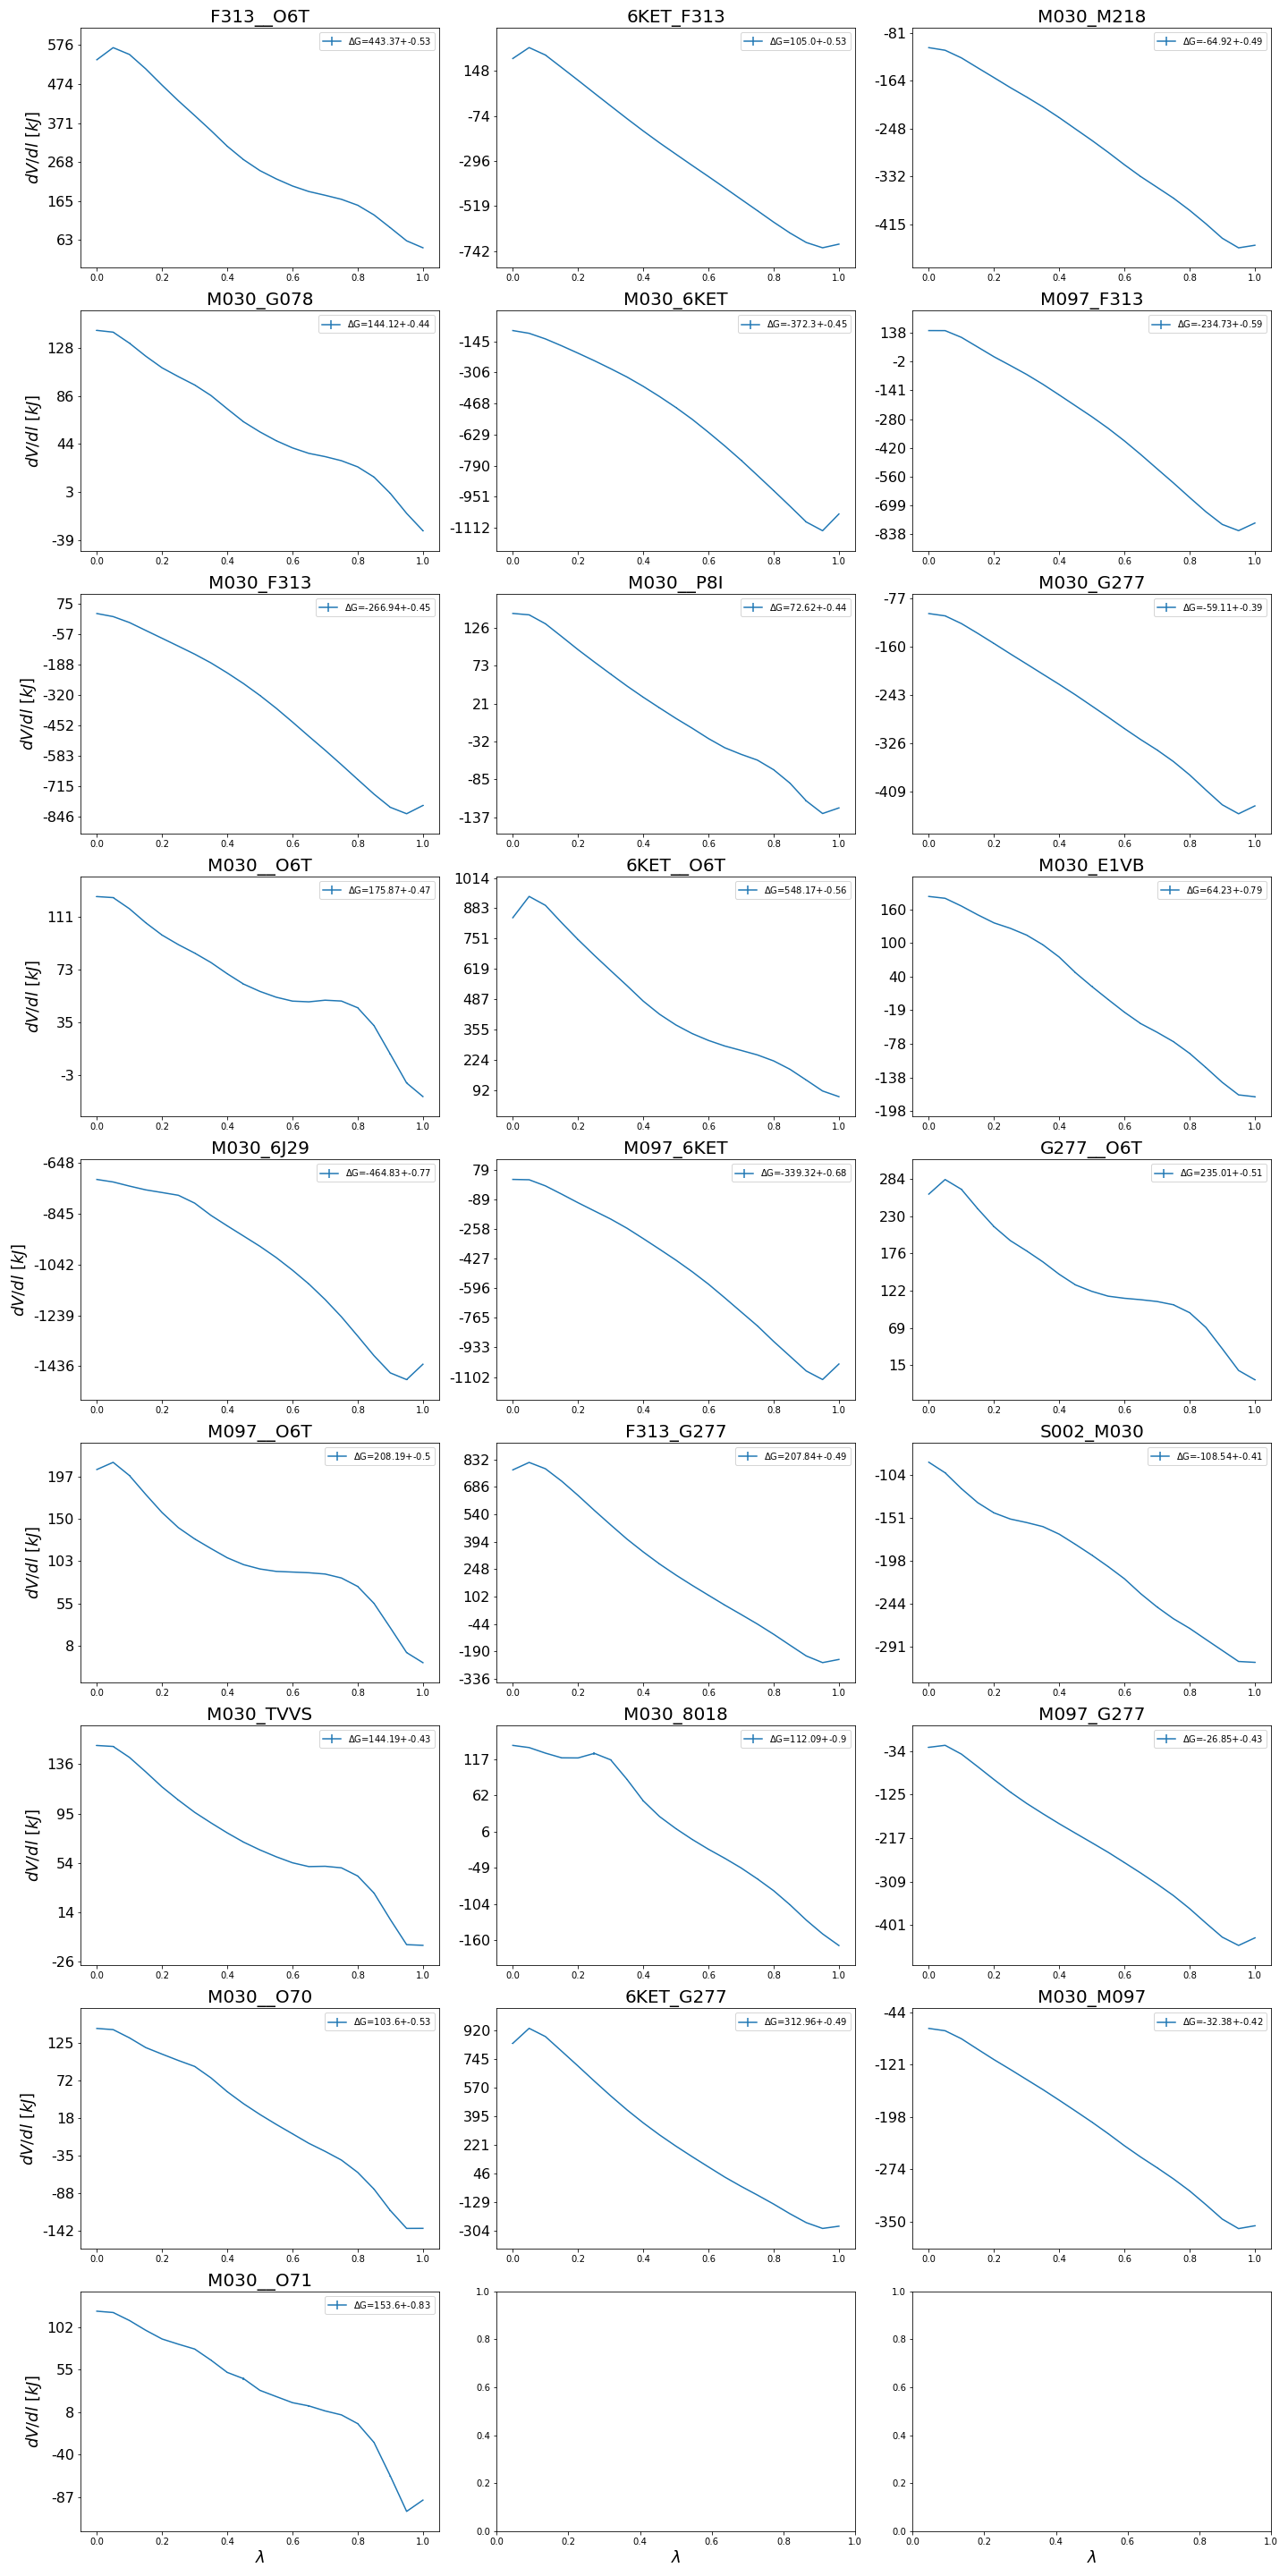
\includegraphics[width=0.65\textwidth]{fig/SI/dG_convergence/TI_water_lambda_curves.png}
    \caption{Pairwise TI-Water $\lambda$-curves}
    \label{SIfig:TI_water_curve}
\end{figure}

\begin{figure}
    \centering
    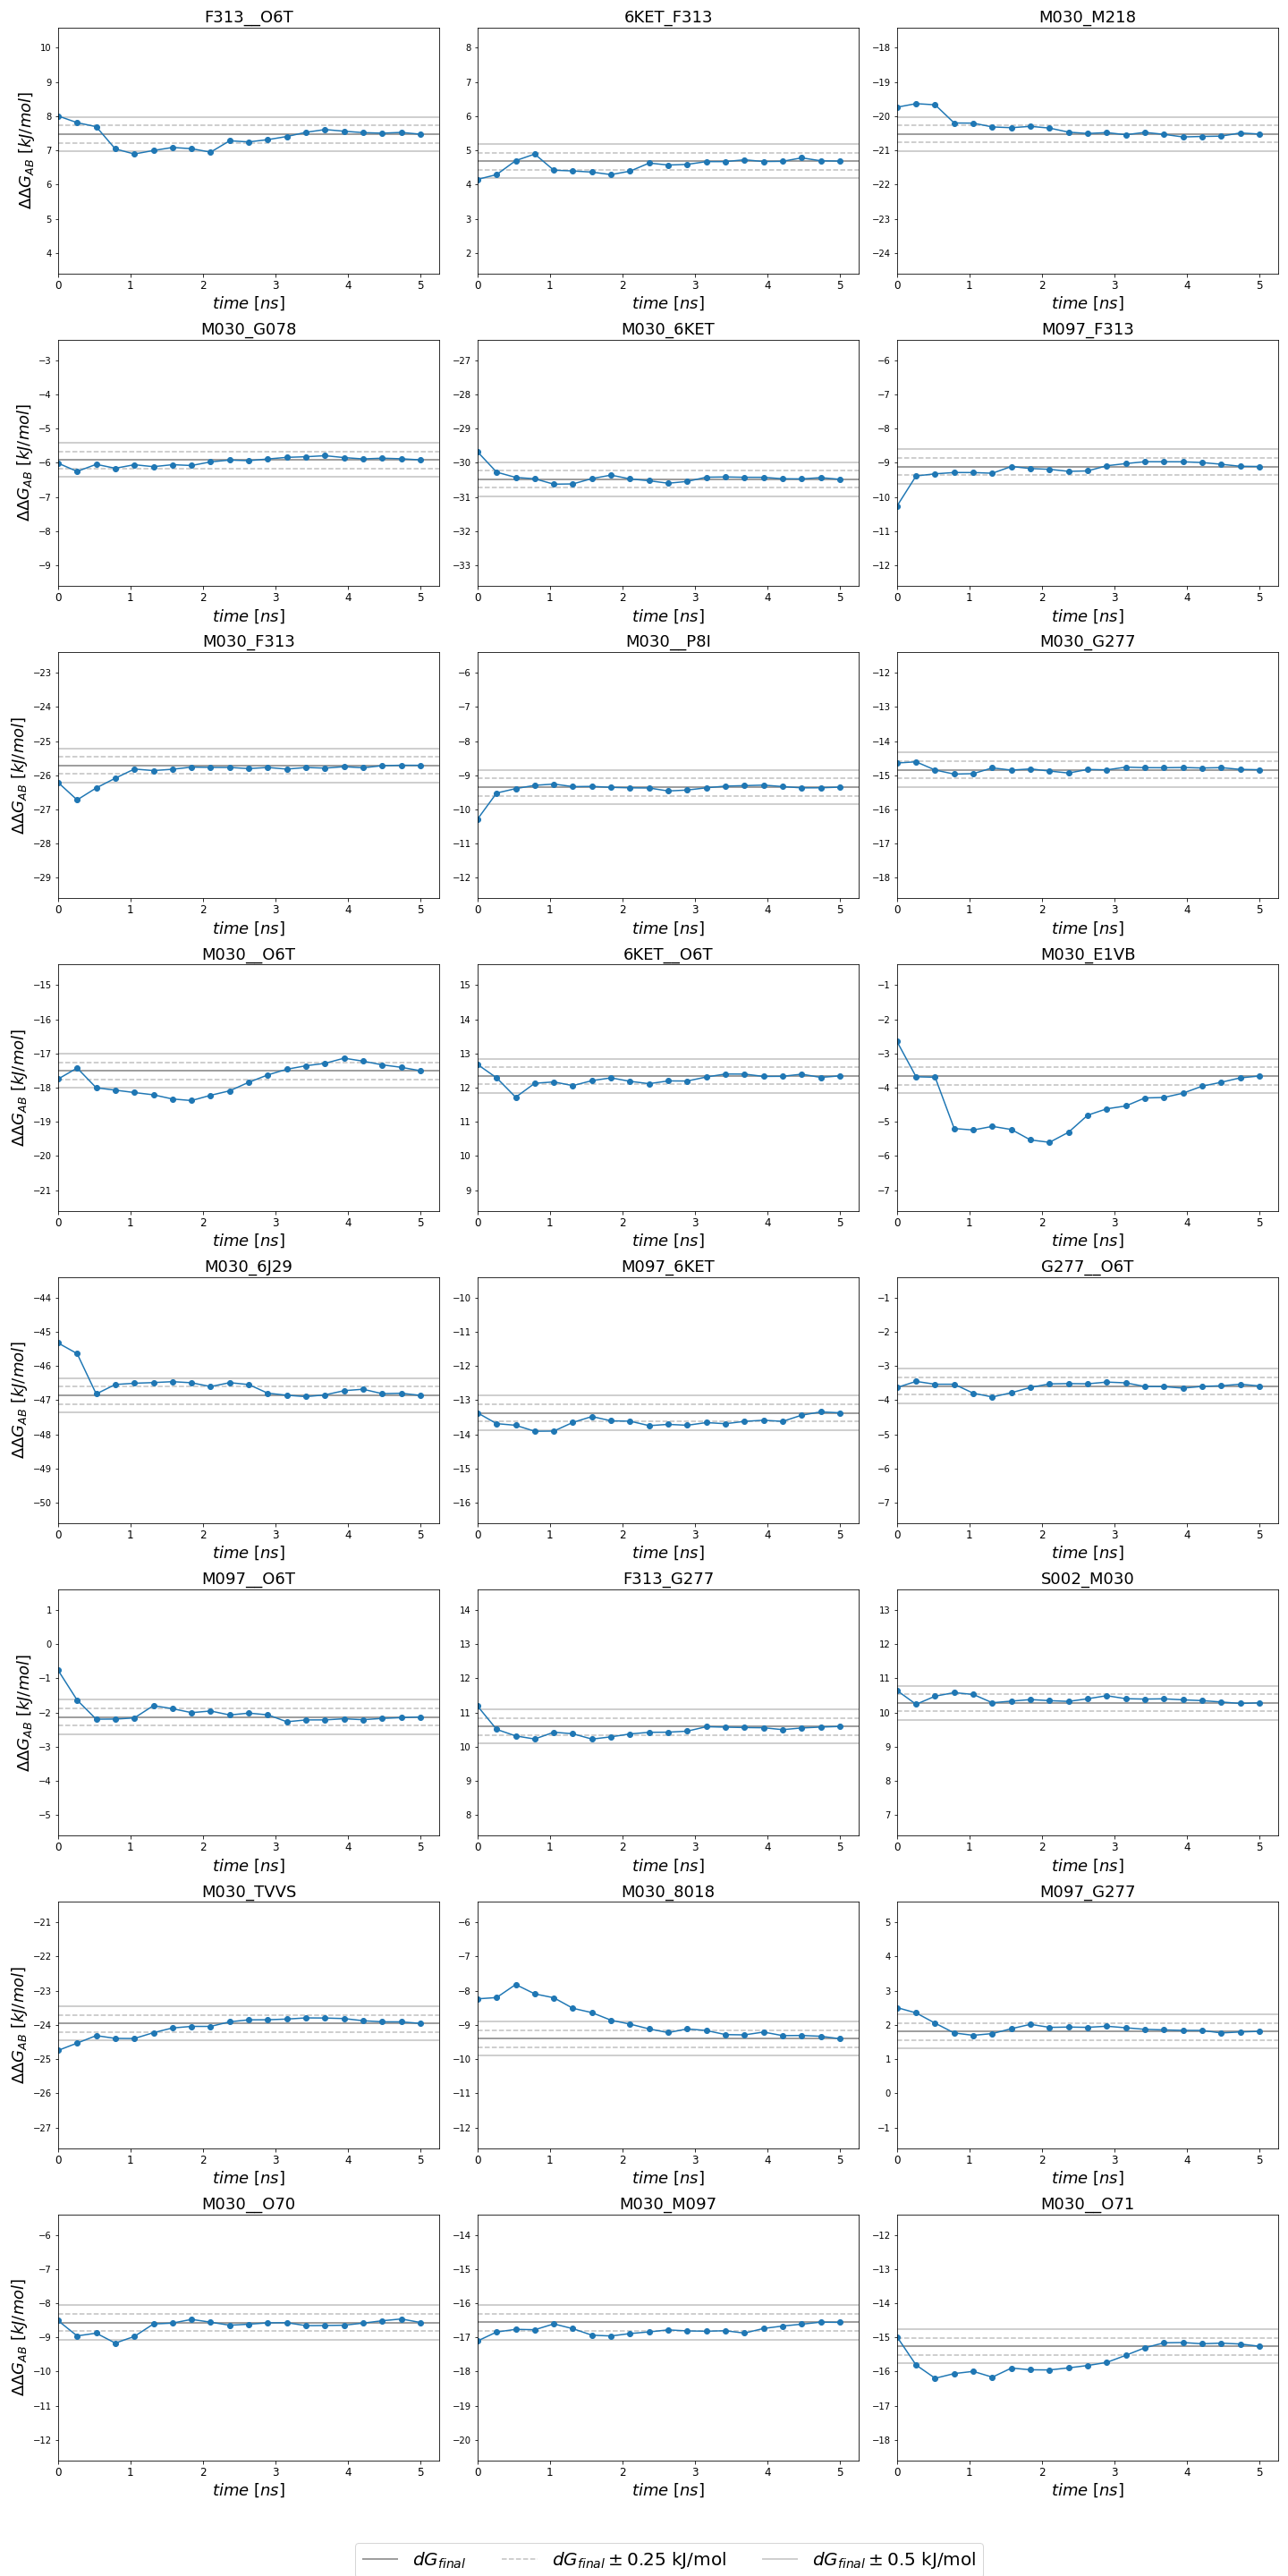
\includegraphics[width=0.65\textwidth]{fig/SI/dG_convergence/ddG_TI_convergence.png}
    \caption{time convergence of the pairwise TI free energy difference calculation of star-map Graph approach for ddG. (see Figure \ref{SIfig: Pairwise_TI_M030_Graph})}
    \label{fig: SI_figure df_convergence_TI}
\end{figure}
